\documentclass[a4paper,oneside,11pt]{book}

% Package dasar
\usepackage[utf8]{inputenc}     % untuk karakter UTF-8
\usepackage[T1]{fontenc}        % encoding font
\usepackage{amsmath}
\usepackage{amssymb}
\usepackage{graphicx}
\usepackage{titling}
\usepackage{titlesec}
\usepackage[backend=biber,style=ieee]{biblatex}
\addbibresource{ref.bib}
\setcounter{biburllcpenalty}{7000}
\setcounter{biburlucpenalty}{8000}

% Package tambahan untuk layout dan formatting
\usepackage{geometry}           % untuk margin
\usepackage{setspace}           % untuk spasi baris
\usepackage{fancyhdr}           % untuk header/footer
\usepackage{hyperref}           % untuk link dan bookmark
\usepackage{xurl}               % agar URL panjang bisa wrap/pindah baris dengan rapi
\usepackage{listings}           % untuk code Python
\usepackage{xcolor}             % untuk warna
\usepackage{float}              % untuk posisi gambar
\usepackage{tocloft}            % Untuk membuat daftar isi menampilkan "Bab 1. Pendahuluan" instead of "1. Pendahuluan",
\usepackage{lipsum}             % untuk lorem ipsum
\usepackage{indentfirst}        % untuk indent paragraf pertama
\usepackage{enumitem}           % untuk kustomisasi penomoran list (A., B., dst)
\usepackage{multirow}           % untuk sel tabel multi-baris

% Pengaturan layout
\geometry{left=3cm, right=2cm, top=2cm, bottom=2cm}
\onehalfspacing  % spasi 1.5

% Penomoran section dengan huruf kapital (A, B, C, ...)
\renewcommand{\thesection}{\Alph{section}}
\renewcommand{\thesubsection}{\thesection.\arabic{subsection}}
\renewcommand{\thesubsubsection}{\thesubsection.\arabic{subsubsection}}

% Penomoran figure dan table mengikuti section (misal, Gambar A.1, Tabel A.1, ...)
\renewcommand{\thefigure}{\thesection.\arabic{figure}}
\renewcommand{\thetable}{\thesection.\arabic{table}}
\renewcommand{\theHfigure}{\theHsection.\arabic{figure}}
\renewcommand{\theHtable}{\theHsection.\arabic{table}}
\makeatletter
\@addtoreset{figure}{section}
\@addtoreset{table}{section}
\makeatother

% Format chapter
\titleformat{\chapter}[hang]
  {\normalfont\huge\bfseries\centering}{\chaptertitlename\ \thechapter.}{1em}{}

% Format code Python
% --- VS Code-like code style (dark) ---
\definecolor{vscodeBg}{HTML}{1E1E1E}
\definecolor{vscodeFg}{HTML}{D4D4D4}
\definecolor{vscodeKeyword}{HTML}{569CD6}
\definecolor{vscodeString}{HTML}{CE9178}
\definecolor{vscodeComment}{HTML}{6A9955}
\definecolor{vscodeNumber}{HTML}{858585}
\definecolor{vscodeRule}{HTML}{3C3C3C}

\lstdefinestyle{vscode-dark}{
  language=Python,
  basicstyle=\ttfamily\small\color{vscodeFg},
  backgroundcolor=\color{vscodeBg},
  keywordstyle=\color{vscodeKeyword}\bfseries,
  commentstyle=\color{vscodeComment},
  stringstyle=\color{vscodeString},
  numbers=left,
  numberstyle=\tiny\color{vscodeNumber},
  frame=single,
  rulecolor=\color{vscodeRule},
  breaklines=true,
  showstringspaces=false,
  columns=fullflexible,
  keepspaces=true,
  tabsize=2,
  xleftmargin=2cm,
  xrightmargin=1cm,
  captionpos=b,
  morekeywords={np, pd, joblib, Flask, Path, Pipeline, StandardScaler, LabelEncoder, DecisionTreeClassifier, RandomForestClassifier, AdaBoostClassifier, LogisticRegression, KNeighborsClassifier, DataFrame, Series, read_csv, dropna, drop, replace, concat, fit, fit_transform, predict, predict_proba, dump, load, route, render_template, redirect, url_for, request}
}

\lstset{style=vscode-dark}

% Pengaturan hyperref
\hypersetup{
    colorlinks=true,
    linkcolor=black,
    filecolor=magenta,
    linktoc=all,
    urlcolor=blue,
    citecolor=red
}

% Info dokumen
\newcommand{\Pertemuan}{10 \& 11}
\newcommand{\Materi}{Model Deployment}
\title{Laporan Praktikum \\ Praktikum Penambangan Data\\
Pertemuan \Pertemuan\\
\Materi}
\newcommand{\NamaMahasiswa}{Muhammad Fauzan Putra Trisuladana}
\newcommand{\NIMMahasiswa}{24/538699/SV/24524}
\newcommand{\KelasMahasiswa}{A1}
\newcommand{\DosenPengampu}{Dr. Imam Fahrurrozi, S.T., M.Cs.}

\author{\NamaMahasiswa\\\NIMMahasiswa}

\begin{document}

% Title Page
\begin{titlingpage} 
  \begin{center}

    \vspace{4cm}
    \begin{Large} 
      \textbf{\thetitle} \\
    \end{Large}
    \vspace{2cm}
    
    
\includegraphics[height=8cm]{resource/lambang ugm.png}\\ 
    \vspace{2cm}
    
    \textbf{Disusun oleh:}\\[0.8em]
    \begin{minipage}{0.8\textwidth}
      \raggedright
      \begin{large}
        \begin{tabular}{@{}l@{\hspace{1.5em}}c@{\hspace{1.5em}}l@{}}
          Nama           & : & \NamaMahasiswa  \\
          NIM            & : & \NIMMahasiswa   \\
          Kelas          & : & \KelasMahasiswa \\
          Dosen Pengampu & : & \DosenPengampu  \\
        \end{tabular}
      \end{large}
    \end{minipage}
    
    \vspace{2cm}
    \begin{Large}
      \textbf{Program Studi D-IV Teknologi Rekayasa Perangkat Lunak} \\
      \textbf{Departemen Teknik Elektro dan Informatika} \\
      \textbf{Sekolah Vokasi}\\
      \textbf{Universitas Gadjah Mada}\\
      \textbf{Yogyakarta}\\
      \textbf{2026}\\
    \end{Large}
    
  \end{center}
\end{titlingpage}

% Header/Footer
\pagestyle{fancy}
\fancyhf{}            % kosongkan header/footer default
\renewcommand{\headrulewidth}{0pt} % hilangkan garis header (atas)
\renewcommand{\footrulewidth}{0pt} % pastikan tidak ada garis footer
\fancyfoot[C]{\thepage} % taruh nomor halaman di footer tengah

% Pastikan halaman dengan style 'plain' (mis. ToC/List) juga tanpa garis atas
\fancypagestyle{plain}{
  \fancyhf{}
  \renewcommand{\headrulewidth}{0pt}
  \renewcommand{\footrulewidth}{0pt}
  \fancyfoot[C]{\thepage}
}

% --- Styling Judul Daftar Isi, Gambar, dan Kode ---
\renewcommand{\cfttoctitlefont}{\hfill\normalfont\LARGE\bfseries}
\renewcommand{\cftaftertoctitle}{\hfill}
\renewcommand{\cftbeforetoctitleskip}{1em}
\renewcommand{\cftaftertoctitleskip}{1.5em}

% --- Format Bab di Daftar Isi ---
\renewcommand{\cftchappresnum}{Bab~}
\renewcommand{\cftchapaftersnum}{.}
\renewcommand{\cftchapnumwidth}{3.5em}
\renewcommand{\cftchapfont}{\bfseries}
\renewcommand{\cftchappagefont}{\bfseries}

% --- Spasi dan Estetika ---
\setlength{\cftbeforechapskip}{0.8em} % jarak antar bab
\setlength{\cftbeforesecskip}{0.2em}  % jarak antar subbab
\renewcommand{\cftsecfont}{\normalfont}
\renewcommand{\cftsubsecfont}{\normalfont}

% --- Judul Lokal ---
\renewcommand{\contentsname}{\centering Daftar Isi}
\renewcommand{\listfigurename}{\centering Daftar Gambar}
\renewcommand{\lstlistlistingname}{\centering Daftar Kode}

% --- Gaya Daftar Gambar dan Daftar Kode ---
\renewcommand{\cftloftitlefont}{\hfill\normalfont\LARGE\bfseries}
\renewcommand{\cftafterloftitle}{\hfill}

\tableofcontents

\newpage
% Daftar Gambar
\listoffigures

\newpage
% Daftar Listing
\lstlistoflistings

% --- Halaman Laporan Pertemuan ---
\newpage
\begin{center}
  \textbf{\LARGE Pertemuan \Pertemuan\\
  {[{\Materi}]}}
\end{center}

\section{Tujuan Praktikum}
\begin{enumerate}[label=\Alph*.]
  \item Mahasiswa mampu memahami konsep dasar dan arsitektur \textit{model deployment} dalam siklus hidup \textit{machine learning} (\textit{ML Lifecycle}).
  \item Mahasiswa mampu melakukan \textit{serialization} (penyimpanan) dan \textit{deserialization} (pemuatan) model \textit{machine learning} menggunakan pustaka \texttt{joblib} ke dalam format biner terstandarisasi (\texttt{.model} atau \texttt{.joblib}).
  \item Mahasiswa dapat merancang dan membangun layanan web (\textit{Web Service}) menggunakan \textit{framework} Flask berbasis antarmuka WSGI, rute endpoint, dan templat formulir HTML.
  \item Mahasiswa dapat merancang dan membangun aplikasi data (\textit{Data Application}) interaktif menggunakan \textit{framework} Streamlit dengan komponen widget visual, kontainer tata letak, dan arsitektur eksekusi \textit{script rerun}.
  \item Mahasiswa mampu mengimplementasikan manajemen \textit{state} interaktif (\texttt{st.session\_state}) serta optimasi \textit{caching} (\texttt{@st.cache\_resource} dan \texttt{@st.cache\_data}) untuk menjamin efisiensi inferensi model pada aplikasi Streamlit.
  \item Mahasiswa mampu melakukan evaluasi komparatif multi-model dan menganalisis perbedaan paradigma penayangan antara \textit{Web Service} (Flask) dan \textit{Data Application} (Streamlit).
\end{enumerate}

\section{Dasar Teori}

\subsection{Python dan Virtual Environment}
\par Python adalah bahasa pemrograman tingkat tinggi yang bersifat \textit{open-source} dan bertipe \textit{general-purpose} dengan filosofi desain yang mengutamakan \textit{code readability} \cite{telkom_python, dicoding_python}. Ketersediaan ekosistem pustaka komputasi ilmiah, pemodelan statistik, serta pengembangan layanan web menjadikan Python sebagai bahasa standar dalam alur kerja \textit{data mining} dari tahap eksplorasi hingga \textit{deployment} produksi \cite{python_docs, han2022data}.
\par Dalam pengembangan aplikasi Python untuk kebutuhan produksi, penggunaan \textit{virtual environment} sangat dianjurkan guna mengisolasi instalasi pustaka suatu proyek dari lingkungan global sistem operasi \cite{python_packaging_venv}. Pembuatan lingkungan terisolasi menggunakan modul standar \texttt{venv} maupun manajer paket modern seperti \texttt{uv} dari Astral memastikan keseragaman versi \textit{interpreter} Python dan pustaka pendamping antara tahap pembuatan model dan tahap penayangan layanan web \cite{python_packaging_venv, astral_uv}. Konsistensi versi pustaka ini mencegah terjadinya konflik dependensi maupun galat ketidakcocokan struktur internal objek saat model dimuat kembali di sisi \textit{server} \cite{scikit_persistence}.

\subsection{NumPy, Pandas, dan Scikit-Learn}
\par NumPy atau Numerical Python adalah pustaka dasar komputasi numerik pada Python yang menyediakan struktur array multidimensi \texttt{ndarray} dengan pengelolaan memori yang efisien serta dukungan operasi matematis tervektorisasi \cite{dqlab_numpy, ruangguru_numpy}. Di atas fondasi NumPy, pustaka Pandas menyediakan struktur data \texttt{Series} dan \texttt{DataFrame} yang memfasilitasi pembacaan berkas CSV, pembersihan data, seleksi kolom atribut, serta penyusunan satu baris data input pengguna dari formulir web menjadi struktur tabel dua dimensi yang siap diumpankan ke model prediktif \cite{datacamp_pandas, dqlab_pandas}.
\par Adapun Scikit-Learn merupakan pustaka \textit{machine learning} terpadu pada ekosistem Python yang menyediakan beragam algoritma \textit{supervised} maupun \textit{unsupervised learning}, utilitas \textit{data preprocessing}, komposisi \texttt{Pipeline}, hingga modul evaluasi metrik dengan antarmuka metode objek yang seragam seperti fungsi \path{fit()}, \path{transform()}, \path{predict()}, dan \path{predict_proba()} \cite{pedregosa2011scikit, scikit_classification}.

\subsection{Machine Learning dan Siklus Hidup Pengembangannya (ML Lifecycle)}
\par Machine Learning (ML) adalah cabang utama kecerdasan buatan yang berfokus pada perancangan algoritma induktif yang mampu mempelajari pola statistik dari data historis untuk menghasilkan prediksi atau keputusan pada data baru tanpa diprogram secara eksplisit \cite{aws_ml, dqlab_ml}. Pengembangan sistem \textit{machine learning} bukanlah aktivitas satu kali jalan yang berhenti setelah model memperoleh skor akurasi di lingkungan eksperimen, melainkan sebuah siklus berkesinambungan yang dikenal sebagai \textit{Machine Learning Lifecycle} atau \textit{ML Pipeline} \cite{geeksforgeeks_ml_lifecycle, huyen2022designing}.
\par Secara sistematis, tahapan siklus hidup pengembangan \textit{machine learning} mencakup sepuluh fase yang saling terhubung \cite{geeksforgeeks_ml_lifecycle, kreuzberger2023mlops}:
\begin{enumerate}[label=\arabic*.]
  \item \textbf{\textit{Problem Definition}:} Merumuskan permasalahan bisnis atau teknis yang hendak diselesaikan beserta sasaran prediksi dan metrik keberhasilannya.
  \item \textbf{\textit{Data Collection}:} Mengumpulkan data mentah yang relevan dari berbagai sumber seperti sensor perangkat keras, rekam medis laboratorium, atau basis data.
  \item \textbf{\textit{Data Cleaning \& Preprocessing}:} Membersihkan \textit{missing values}, menangani derau data, serta menyamakan format dan skala representasi atribut.
  \item \textbf{\textit{Exploratory Data Analysis} (EDA):} Menganalisis distribusi variabel, korelasi antarfitur, dan proporsi kelas secara statistik maupun visual.
  \item \textbf{\textit{Feature Engineering \& Selection}:} Mengekstraksi, mengodekan, dan memilih himpunan fitur yang paling informatif bagi pemodelan.
  \item \textbf{\textit{Model Selection}:} Memilih kandidat algoritma pembelajaran mesin yang sesuai dengan karakteristik distribusi data dan jenis target.
  \item \textbf{\textit{Model Training}:} Melatih kandidat model menggunakan \textit{training set} agar mempelajari parameter pemetaan fitur terhadap target.
  \item \textbf{\textit{Model Evaluation and Tuning}:} Menguji performa generalisasi model pada \textit{testing set} serta melakukan penalaan hiperparameter terbaik.
  \item \textbf{\textit{Model Deployment}:} Mengintegrasikan model terlatih ke dalam lingkungan produksi atau layanan aplikasi agar dapat diakses oleh pengguna akhir.
  \item \textbf{\textit{Model Monitoring \& Maintenance}:} Memantau kinerja model secara berkelanjutan terhadap pergeseran distribusi data (\textit{data drift}) dan memperbarui model secara berkala.
\end{enumerate}
\par Tanpa melewati tahap kesembilan berupa \textit{model deployment}, sebuah model yang telah dilatih dan dievaluasi dengan akurasi tinggi hanya bersifat statis di komputer pengembang dan belum memberikan nilai guna praktis bagi pengguna lain \cite{huyen2022designing, kreuzberger2023mlops}.

\subsection{Data Preprocessing dan Pipeline}
\par \textit{Data preprocessing} adalah tahapan penting untuk mengubah data mentah menjadi format numerik yang bersih dan terstandarisasi sebelum dipelajari oleh algoritma \cite{techtarget_preprocessing, trivusi_preprocessing}. Dalam pemodelan data tabular, tahapan ini meliputi penghapusan baris bernilai kosong (\path{dropna()}), pengodean label kategorikal menjadi bilangan bulat melalui \path{LabelEncoder}, penyesuaian urutan kolom fitur, serta penyetaraan skala variabel numerik menggunakan \path{StandardScaler} dengan rumus skor baku $z = (x - \mu) / \sigma$ \cite{pedregosa2011scikit, han2022data}.
\par Ketika sebuah model hendak di-\textit{deploy} ke dalam layanan web, seluruh langkah transformasi prapemrosesan yang diterapkan pada data pelatihan wajib diterapkan secara identik pada data masukan baru saat inferensi \cite{huyen2022designing, scikit_pipeline}. Objek \texttt{Pipeline} pada Scikit-Learn memungkinkan penggabungan tahapan transformasi seperti \texttt{StandardScaler} dan objek \textit{classifier} ke dalam satu kesatuan estimator tunggal \cite{scikit_pipeline}. Penggunaan \texttt{Pipeline} mencegah terjadinya \textit{data leakage} selama evaluasi serta menjamin bahwa ketika objek \textit{pipeline} disimpan dan dimuat kembali di aplikasi web, setiap input mentah dari pengguna akan melewati parameter penskalaan yang persis sama sebelum diprediksi oleh model \cite{scikit_pipeline, scikit_persistence}.

\subsection{Classification dan Algoritma Klasifikasi}
\par \textit{Classification} adalah tugas dalam paradigma \textit{supervised learning} yang bertujuan memetakan vektor fitur masukan ke dalam salah satu label kategori diskret berdasarkan pola dari data berlabel \cite{retnoningsih2020mengenal, roihan2020pemanfaatan}. Permasalahan klasifikasi dapat berupa \textit{binary classification} dengan dua kelas keluaran---seperti deteksi keterisian ruangan antara kosong atau terisi \cite{candanedo2016accurate}---maupun \textit{multiclass classification} yang mencakup lebih dari dua kategori---seperti klasifikasi tahapan klinis penyakit hati Hepatitis C ke dalam kategori donor darah sehat, hepatitis, fibrosis, dan sirosis \cite{hoffmann2018using, ibm_classification}.
\par Lima algoritma klasifikasi populer yang diimplementasikan dan dievaluasi pada praktikum ini meliputi \cite{scikit_classification, han2022data}:
\begin{enumerate}[label=\arabic*.]
  \item \textbf{Decision Tree:} Algoritma berbasis struktur pohon hierarkis yang mempartisi ruang fitur secara rekursif pada setiap \textit{internal node} berdasarkan kriteria kemurnian kelas seperti \textit{Gini Impurity} atau \textit{Information Gain} berbasis \textit{Entropy}, hingga mencapai keputusan label kelas pada \textit{leaf node} \cite{ibm_decision_tree, han2022data}.
  \item \textbf{Logistic Regression:} Algoritma klasifikasi linear yang memodelkan probabilitas keanggotaan suatu kelas menggunakan kombinasi linear fitur masukan yang dipetakan melalui fungsi logistik Sigmoid \cite{ibm_logistic_regression}.
  \item \textbf{K-Nearest Neighbors (KNN):} Algoritma \textit{instance-based learning} non-parametrik yang menentukan kelas suatu sampel uji berdasarkan suara mayoritas dari $k$ tetangga terdekatnya pada ruang jarak Euclidean \cite{ibm_knn}.
  \item \textbf{Random Forest:} Algoritma ansambel berbasis \textit{bagging} yang membangun banyak pohon keputusan secara paralel di atas sampel \textit{bootstrap} dan subset fitur acak, lalu menggabungkan prediksinya melalui \textit{majority voting} guna menekan variansi dan mencegah \textit{overfitting} \cite{ibm_random_forest}.
  \item \textbf{AdaBoost:} Algoritma ansambel berbasis \textit{boosting} yang melatih rangkaian \textit{weak learners} secara sekuensial dengan meningkatkan bobot sampel yang salah diklasifikasikan pada iterasi sebelumnya \cite{scikit_adaboost}.
\end{enumerate}

\subsection{Metrik Evaluasi Classification}
\par Pengujian kuantitatif kualitas prediksi model klasifikasi dilakukan menggunakan \textit{confusion matrix} yang memetakan perbandingan antara label aktual dan label hasil prediksi model ke dalam empat komponen: \textit{True Positive} ($TP$), \textit{True Negative} ($TN$), \textit{False Positive} ($FP$), dan \textit{False Negative} ($FN$) \cite{trivusi_confusion_matrix, fawcett2006introduction}. Dari keempat komponen tersebut, diturunkan empat metrik evaluasi utama sebagaimana dirumuskan pada Persamaan \eqref{eq:metrics-all} \cite{scikit_metrics, dqlab_classification_metrics}:
\begin{equation}
  \text{Accuracy} = \frac{TP + TN}{TP + TN + FP + FN}, \quad
  \text{Precision} = \frac{TP}{TP + FP}, \quad
  \text{Recall} = \frac{TP}{TP + FN}
  \label{eq:metrics-all}
\end{equation}
\par Adapun keseimbangan harmonik antara nilai \textit{precision} dan \textit{recall} diukur menggunakan metrik \textit{F1-score} sebagaimana dinyatakan pada Persamaan \eqref{eq:f1-metric} \cite{normawati2021implementasi, dqlab_classification_metrics}:
\begin{equation}
  \text{F1-Score} = 2 \times \frac{\text{Precision} \times \text{Recall}}{\text{Precision} + \text{Recall}}
  \label{eq:f1-metric}
\end{equation}
Pada dataset yang memiliki ketimpangan jumlah sampel antarkelas (\textit{imbalanced class distribution}), perhitungan rata-rata makro (\textit{macro average}) pada \textit{precision}, \textit{recall}, dan \textit{F1-score} memberikan bobot yang setara bagi setiap kelas sehingga performa model pada kelas minoritas tetap terukur secara objektif \cite{scikit_metrics, fawcett2006introduction}.

\subsection{Model Serialization dan Deserialization}
\par Objek model \textit{machine learning} yang telah selesai dilatih pada dasarnya tersimpan sebagai struktur data sementara di dalam memori utama (RAM) dan akan hilang ketika eksekusi skrip Python dihentikan \cite{scikit_persistence}. Agar model tersebut dapat digunakan kembali oleh aplikasi lain tanpa harus mengulangi proses pelatihan dari awal, diperlukan mekanisme \textit{model serialization}, yakni proses mengubah struktur objek model di dalam memori menjadi urutan aliran \textit{byte} untuk disimpan ke dalam berkas fisik seperti berekstensi \texttt{.pkl}, \texttt{.model}, atau \texttt{.joblib} \cite{python_pickle, joblib_docs}.
\par Sebaliknya, proses membaca kembali berkas biner tersebut dari media penyimpanan ke dalam memori aplikasi guna membentuk ulang objek model utuh yang siap menjalankan fungsi \path{predict()} disebut \textit{deserialization} \cite{python_pickle, scikit_persistence}. Dalam ekosistem Python dan Scikit-Learn, terdapat dua pustaka utama untuk keperluan ini, yakni modul bawaan \texttt{pickle} serta pustaka \texttt{joblib} melalui fungsi \path{joblib.dump()} dan \path{joblib.load()} \cite{python_pickle, joblib_docs}. Pustaka \texttt{joblib} lebih direkomendasikan untuk objek estimator Scikit-Learn karena memiliki efisiensi serialisasi yang jauh lebih tinggi ketika menangani objek yang menyimpan struktur array NumPy berukuran besar secara internal \cite{scikit_persistence, joblib_docs}.

\subsection{Model Deployment dan Arsitektur Client-Server}
\par \textit{Model deployment} merupakan proses integrasi model \textit{machine learning} yang telah terlatih ke dalam lingkungan operasional sehingga model beralih dari artefak eksperimen statis menjadi layanan aktif yang siap melayani permintaan prediksi dari pengguna akhir maupun sistem perangkat lunak lain \cite{huyen2022designing, kreuzberger2023mlops}. Meskipun terdapat berbagai skema penayangan model seperti penanaman langsung di perangkat (\textit{embedded deployment}) atau pemrosesan terjadwal (\textit{batch prediction}), pola yang paling luas dan fleksibel digunakan pada aplikasi modern adalah arsitektur \textit{client-server} berbasis layanan web atau RESTful API \cite{fielding2000architectural, huyen2022designing}.
\par Pada skema arsitektur \textit{client-server} untuk inferensi model melalui layanan web, alur pertukaran data berlangsung dalam lima tahapan terstruktur \cite{grinberg2018flask, huyen2022designing}:
\begin{enumerate}[label=\arabic*.]
  \item \textbf{\textit{Web Service}:} Aplikasi \textit{server} menyediakan alamat Uniform Resource Locator (URL) yang dapat diakses melalui jaringan untuk menjembatani komunikasi antara pengguna di sisi luar dan logika model Python di sisi internal.
  \item \textbf{\textit{API Endpoint}:} Permintaan data masukan dari \textit{client}---baik melalui peramban web menggunakan formulir HTML \texttt{POST} maupun aplikasi penguji API seperti Postman atau \texttt{curl}---diterima oleh rute pintu gerbang spesifik, misalnya pada alamat \texttt{/tabular/result/} atau \texttt{/predict}.
  \item \textbf{\textit{Web Server Request Processing}:} Layanan web mengekstraksi parameter input yang dikirimkan oleh \textit{client}, memvalidasi nilai masukan, mengonversi tipe data teks menjadi numerik, serta menyusun urutan kolom fitur ke dalam objek \texttt{DataFrame} agar sesuai dengan skema input model.
  \item \textbf{\textit{Model Loading \& Inference}:} Aplikasi memuat berkas model hasil serialisasi yang telah dilatih sebelumnya, lalu mengeksekusi perhitungan matematis inferensi untuk menghasilkan label prediksi beserta estimasi nilai probabilitasnya.
  \item \textbf{\textit{Response}:} Hasil prediksi dikirimkan kembali oleh \textit{server} kepada \textit{client}, baik dalam bentuk muatan terstruktur JavaScript Object Notation (JSON) untuk konsumsi antar-program maupun dirender ke dalam halaman antarmuka HTML yang informatif bagi pengguna manusia.
\end{enumerate}

\subsection{Flask Framework dan WSGI}
\par Flask adalah \textit{micro-web framework} berbahasa Python yang dirancang oleh Armin Ronacher di bawah naungan Pallets Projects dengan mengandalkan pustaka peralatan HTTP Werkzeug serta mesin templat Jinja2 \cite{grinberg2018flask, flask_quickstart}. Flask dikategorikan sebagai \textit{micro-framework} karena menjaga inti kerangka kerjanya tetap ringan, ringkas, dan modular tanpa memaksakan ketergantungan bawaan terhadap lapisan abstraksi basis data seperti Object-Relational Mapping (ORM) atau struktur direktori yang kaku \cite{grinberg2018flask}. Kesederhanaan ini menjadikan Flask sangat populer digunakan oleh praktisi data untuk membungkus model \textit{machine learning} menjadi layanan API maupun aplikasi \textit{dashboard} prediktif secara cepat \cite{huyen2022designing, flask_quickstart}.
\par Dalam pembuatan aplikasi Flask, instansiasi objek utama dilakukan melalui pemanggilan \path{app = Flask(__name__)}, diikuti pendefinisian \textit{decorator} \path{@app.route()} guna memetakan suatu alamat URL ke fungsi penanganan (\textit{view function}) \cite{flask_quickstart}. Objek \path{request.form} digunakan untuk menangkap pasangan kunci dan nilai yang dikirimkan melalui metode HTTP \texttt{POST}, sedangkan fungsi \path{render_template()} memanggil mesin Jinja2 untuk menyuntikkan variabel hasil prediksi Python secara dinamis ke dalam berkas antarmuka HTML di dalam direktori \path{templates/} \cite{grinberg2018flask}.
\par Untuk melayani permintaan HTTP, Flask mengimplementasikan spesifikasi standar Python Web Server Gateway Interface (WSGI) sebagaimana didefinisikan dalam PEP 3333, yakni antarmuka komunikasi standar antara \textit{web server} dan aplikasi web berbasis Python \cite{pep3333_wsgi}. Saat tahap pengembangan lokal, pemanggilan \texttt{app.run()} atau perintah \texttt{flask run} akan menjalankan \textit{development WSGI server} bawaan Werkzeug \cite{flask_quickstart}. Adapun untuk penayangan di lingkungan produksi yang sesungguhnya, dokumentasi resmi Flask merekomendasikan penggunaan \textit{dedicated production WSGI server} seperti Gunicorn atau uWSGI di balik \textit{reverse proxy} HTTP seperti NGINX atau Apache guna menjamin keamanan, konkurensi, dan stabilitas layanan \cite{flask_deploying, grinberg2018flask}.

\subsection{Streamlit Framework dan Paradigma Data Application}
\par Streamlit adalah \textit{open-source framework} berbasis Python murni yang dirancang khusus untuk memfasilitasi praktisi data dan perekayasa \textit{machine learning} dalam membangun antarmuka web interaktif serta \textit{data dashboard} secara cepat tanpa harus menulis kode HTML, CSS, maupun JavaScript secara manual \cite{streamlit_docs, treveil2020introducing}. Berbeda mendasar dengan arsitektur \textit{Request-Response} per rute URL pada Flask, Streamlit mengadopsi paradigma eksekusi yang dikenal sebagai \textit{Script Rerun} \cite{streamlit_execution_model}. Dalam paradigma ini, setiap kali pengguna berinteraksi dengan sebuah widget antarmuka---seperti mengubah angka pada \texttt{st.number\_input}, memilih opsi \texttt{st.selectbox}, atau menekan tombol \texttt{st.button}---Streamlit secara otomatis mengeksekusi ulang keseluruhan skrip Python dari baris pertama hingga baris terakhir \cite{streamlit_execution_model}. Model reaktif ini memungkinkan antarmuka visual selalu mencerminkan kondisi variabel Python terkini secara deterministik \cite{streamlit_execution_model, huyen2022designing}.
\par Komponen antarmuka Streamlit tersusun secara deklaratif dan terbagi ke dalam empat kategori utama \cite{streamlit_docs}:
\begin{enumerate}[label=\arabic*.]
  \item \textbf{\textit{Output \& Text Display}:} Fungsi penampil teks hierarkis (\texttt{st.title()}, \texttt{st.header()}, \texttt{st.caption()}, \texttt{st.markdown()}), visualisasi metrik ringkas (\texttt{st.metric()}), serta notifikasi umpan balik (\texttt{st.success()}, \texttt{st.info()}, \texttt{st.spinner()}).
  \item \textbf{\textit{Input Widgets}:} Komponen interaktif penerima masukan data pengguna (\texttt{st.number\_input()}, \texttt{st.selectbox()}, \texttt{st.slider()}, \texttt{st.button()}), termasuk pembungkus formulir \texttt{st.form()} bersama tombol aksi \texttt{st.form\_submit\_button()} yang menahan siklus \textit{rerun} hingga seluruh kolom selesai diisi.
  \item \textbf{\textit{Layouts \& Containers}:} Pengorganisasian tata letak antarmuka tingkat lanjut seperti bilah navigasi samping (\texttt{st.sidebar}), pembagian kolom horizontal (\texttt{st.columns()}), panel tab bertingkat (\texttt{st.tabs()}), dan panel yang dapat diciutkan (\texttt{st.expander()}).
  \item \textbf{\textit{Session State \& Caching}:} Mekanisme persistensi nilai variabel lokal lintas siklus \textit{rerun} (\texttt{st.session\_state}) serta pengelolaan memori terdistribusi guna menghindari beban komputasi berulang \cite{streamlit_execution_model, streamlit_caching}.
\end{enumerate}
\par Karena skrip Python dijalankan ulang secara menyeluruh pada setiap interaksi, variabel lokal standar akan terinisialisasi kembali ke nilai default. Untuk mempertahankan data yang dimasukkan pengguna atau status aplikasi, Streamlit menyediakan \texttt{st.session\_state} yang bertindak sebagai kamus global per sesi pengguna \cite{streamlit_execution_model}. Selain itu, pemuatan berkas model biner serialisasi (\texttt{.model} atau \texttt{.joblib}) dari media penyimpanan pada setiap siklus \textit{rerun} akan membebani memori dan memperlambat latensi inferensi secara signifikan \cite{streamlit_caching}. Oleh karena itu, dekorator \texttt{@st.cache\_resource} diterapkan pada fungsi pemuatan model agar objek model tersimpan secara persisten di memori bersama (\textit{shared global cache}) dan hanya dimuat satu kali selama siklus hidup server \cite{streamlit_caching}. Adapun untuk data tabular, kamus konfigurasi, atau metadata JSON, dekorator \texttt{@st.cache\_data} digunakan untuk meng-cache salinan data yang dapat diserialisasikan secara aman \cite{streamlit_caching}.


\section{Hasil dan Pembahasan}

\par Sesuai dengan tujuan praktikum, berikut adalah hasil eksperimen beserta pembahasan komprehensif mengenai persiapan lingkungan kerja terisolasi, pelatihan serta serialisasi model \textit{machine learning}, perancangan layanan web menggunakan \textit{framework} Flask, pembangunan \textit{data dashboard} interaktif menggunakan \textit{framework} Streamlit, hingga analisis komparatif performa dan paradigma penayangan model pada kedua platform tersebut.

\subsection{Persiapan Lingkungan Kerja dan Struktur Proyek Deployment}

\subsubsection{Pembuatan Virtual Environment dan Instalasi Pustaka}
\lstinputlisting[language=Python, caption={Pembuatan Virtual Environment Python 3.12 dan Instalasi Dependensi Flask}, label={lst:kode-setup-env-1}]{resource/code/setup-env_1.py}
\par \textbf{Output:}
\lstinputlisting[caption={Output Verifikasi Versi Python dan Daftar Paket pada Virtual Environment}, label={lst:out-setup-env-1}]{resource/output/setup-env_1_out.txt}
\par Berdasarkan sintaks pada Kode \ref{lst:kode-setup-env-1}, langkah persiapan diawali dengan membangun \textit{virtual environment} lokal menggunakan perintah \path{uv venv --seed --python 3.12 .venv} agar seluruh pustaka proyek terisolasi di dalam direktori \path{.venv} tanpa mengganggu paket global sistem operasi. Selanjutnya, kelima pustaka utama yang dibutuhkan untuk pemodelan tabular dan layanan web---yaitu \texttt{flask}, \texttt{numpy}, \texttt{scikit-learn}, \texttt{pandas}, dan \texttt{joblib}---diinstal ke dalam lingkungan tersebut tanpa menyertakan paket \texttt{tensorflow[and-gpu]} karena kedua proyek pada praktikum ini menggunakan algoritma klasifikasi tabular berbasis Scikit-Learn. Sebagaimana tertera pada Output \ref{lst:out-setup-env-1}, lingkungan kerja berhasil terkonfigurasi menggunakan \texttt{Python 3.12.16} beserta versi pustaka yang konsisten antara tahap pelatihan dan tahap inferensi, meliputi \texttt{Flask 3.1.3}, \texttt{scikit-learn 1.9.1}, \texttt{pandas 3.1.1}, \texttt{numpy 2.5.4}, \texttt{joblib 1.6.0}, \texttt{Jinja2 3.1.6}, dan \texttt{Werkzeug 3.1.9}.

\subsubsection{Penataan Struktur Direktori Proyek Latihan dan Tugas}
\lstinputlisting[language=Python, caption={Penataan Struktur Direktori Proyek Latihan dan Tugas beserta Pembersihan Starter}, label={lst:kode-setup-struktur-1}]{resource/code/setup-struktur_1.py}
\par \textbf{Output:}
\lstinputlisting[caption={Output Struktur Pohon Direktori Repositori deploy-flask}, label={lst:out-setup-struktur-1}]{resource/output/setup-struktur_1_out.txt}
\par Berdasarkan sintaks pada Kode \ref{lst:kode-setup-struktur-1}, direktori repositori \path{deploy-flask} ditata ulang dengan memisahkan ruang kerja menjadi dua subproyek mandiri, yakni folder \path{latihan/} untuk percobaan modul prediksi penyakit Hepatitis C dan folder \path{tugas/} untuk proyek tugas deteksi keterisian ruangan (\textit{Room Occupancy Detection}). Masing-masing folder dibagi lebih lanjut menjadi subdirektori \path{create_model/} untuk skrip pelatihan serta serialisasi model dan subdirektori \path{web/} untuk kode layanan Flask beserta aset antarmuka \path{static/} dan \path{templates/}. Berkas-berkas bawaan repositori awal yang tidak relevan dengan pemodelan tabular dibersihkan agar struktur proyek tetap ramping. Hasil eksekusi perintah \texttt{find} pada Output \ref{lst:out-setup-struktur-1} memvalidasi bahwa hierarki direktori \path{docs/}, \path{latihan/}, dan \path{tugas/} telah terbentuk secara rapi dan terorganisasi.

\subsection{Implementasi Model Deployment Prediksi Penyakit Hepatitis C dengan Flask}

\subsubsection{Data Preprocessing, Pelatihan, dan Serialisasi Model Decision Tree}
\lstinputlisting[language=Python, caption={Pelatihan dan Serialisasi Model Decision Tree pada Dataset Hepatitis C}, label={lst:kode-latihan-train-hcv-1}]{resource/code/latihan-train-hcv_1.py}
\par \textbf{Output:}
\lstinputlisting[caption={Output Pelatihan dan Penyimpanan Berkas Model \texttt{dt\_model.model}}, label={lst:out-latihan-train-hcv-1}]{resource/output/latihan-train-hcv_1_out.txt}
\par Berdasarkan sintaks pada Kode \ref{lst:kode-latihan-train-hcv-1}, skrip pembuatan model membaca berkas dataset klinis Hepatitis C (\path{hcvdat0.csv}) lalu menjalankan pembersihan baris yang mengandung \textit{missing values} menggunakan metode \path{dropna()}. Kolom indeks \path{Unnamed: 0} dan kolom target \path{Category} dipisahkan dari matriks fitur, kemudian lima label teks pada kolom \path{Category} dipetakan ulang (\textit{relabelling}) menjadi empat kelas bilangan bulat, di mana kategori \texttt{0=Blood Donor} dan \texttt{0s=suspect Blood Donor} digabungkan ke dalam label \texttt{0}, diikuti \texttt{1=Hepatitis} menjadi \texttt{1}, \texttt{2=Fibrosis} menjadi \texttt{2}, serta \texttt{3=Cirrhosis} menjadi \texttt{3}. Atribut kategorikal \path{Sex} dikodekan menjadi numerik menggunakan \path{LabelEncoder()} dan digabungkan kembali di posisi kolom pertama melalui \path{pd.concat([sex_encoded, df_x_num], axis=1)}. Selanjutnya, fungsi \path{train_and_save_decision_tree()} melatih objek \path{DecisionTreeClassifier(random_state=0)} dan mengekspornya ke dalam berkas fisik \path{dt_model.model} menggunakan fungsi \path{joblib.dump()}. Mengacu pada Output \ref{lst:out-latihan-train-hcv-1}, dari $615$ baris dan $14$ kolom data awal tersisa $589$ baris bersih dengan urutan $12$ fitur \texttt{['Sex', 'Age', 'ALB', 'ALP', 'ALT', 'AST', 'BIL', 'CHE', 'CHOL', 'CREA', 'GGT', 'PROT']} serta pemetaan \path{LabelEncoder} \texttt{\{'f': 0, 'm': 1\}}. Model berhasil mencapai \textit{in-sample training accuracy} sebesar $1{,}0000$, dan berkas biner \path{dt_model.model} berukuran $5{,}7\text{ KB}$ telah tersimpan di folder pembuatan model sekaligus disalin ke dalam folder aplikasi web \path{latihan/web/dt_model.model}.

\subsubsection{Perancangan Layanan Web dan Endpoint Inferensi Flask}
\lstinputlisting[language=Python, caption={Implementasi Aplikasi Web Flask dan Endpoint Prediksi Hepatitis C}, label={lst:kode-latihan-flask-app-1}]{resource/code/latihan-flask-app_1.py}
\par \textbf{Output:}
\lstinputlisting[caption={Output Pengujian Endpoint Server Flask Latihan dan Inferensi Prediksi Cirrhosis}, label={lst:out-latihan-flask-app-1}]{resource/output/latihan-flask-app_1_out.txt}
\par Berdasarkan sintaks pada Kode \ref{lst:kode-latihan-flask-app-1}, aplikasi web Flask dibangun dengan memuat berkas model \path{dt_model.model} sekali di tingkat modul melalui \path{joblib.load(MODEL_PATH)} agar objek model langsung siap di memori tanpa perlu dibaca ulang dari cakram pada setiap permintaan HTTP. Dua fungsi bantu, yakni \path{_to_float()} dan \path{_encode_sex()}, dirancang untuk mengonversi nilai string yang diambil dari formulir HTML menjadi tipe \texttt{float} serta menyamakan kode jenis kelamin (\texttt{'m'}/\texttt{'1'} menjadi \texttt{1} dan \texttt{'f'}/\texttt{'0'} menjadi \texttt{0}). Aplikasi menyediakan tiga rute URL: rute akar \path{/} yang mengalihkan pengguna ke halaman utama, rute \path{/tabular/} (\texttt{GET}) yang merender halaman formulir \path{index.html}, serta rute \path{/tabular/result/} (\texttt{POST}) yang menangkap $12$ parameter klinis dari \path{request.form}, menyusunnya ke dalam \path{pd.DataFrame} sesuai konstanta urutan \path{COLUMNS_ORDER}, menjalankan inferensi \path{LOADED_MODEL.predict(df_input)}, memetakan indeks kelas ke nama diagnosis melalui kamus \path{DIAGNOSIS_MAP}, dan merender hasilnya ke templat \path{result.html}. Sebagaimana ditunjukkan pada Output \ref{lst:out-latihan-flask-app-1}, server pengembangan WSGI Flask berjalan di alamat \url{http://127.0.0.1:5000} dan merespons permintaan \texttt{GET /tabular/} maupun pengiriman formulir \texttt{POST /tabular/result/} dengan kode status \texttt{HTTP 200}, di mana kombinasi input uji sesuai modul (\texttt{Age=30}, \texttt{Sex=1}, \texttt{ALB=39}, \texttt{ALP=100}, \texttt{ALT=28}, \texttt{AST=143}, \texttt{BIL=15}, \texttt{CHE=5}, \texttt{CHOL=4}, \texttt{CREA=72}, \texttt{GGT=400}, \texttt{PROT=73}) berhasil menghasilkan keluaran prediksi \texttt{Cirrhosis}.

\subsubsection{Pengujian Antarmuka Web Prediksi Penyakit Hepatitis C}

\begin{figure}[H]
  \centering
  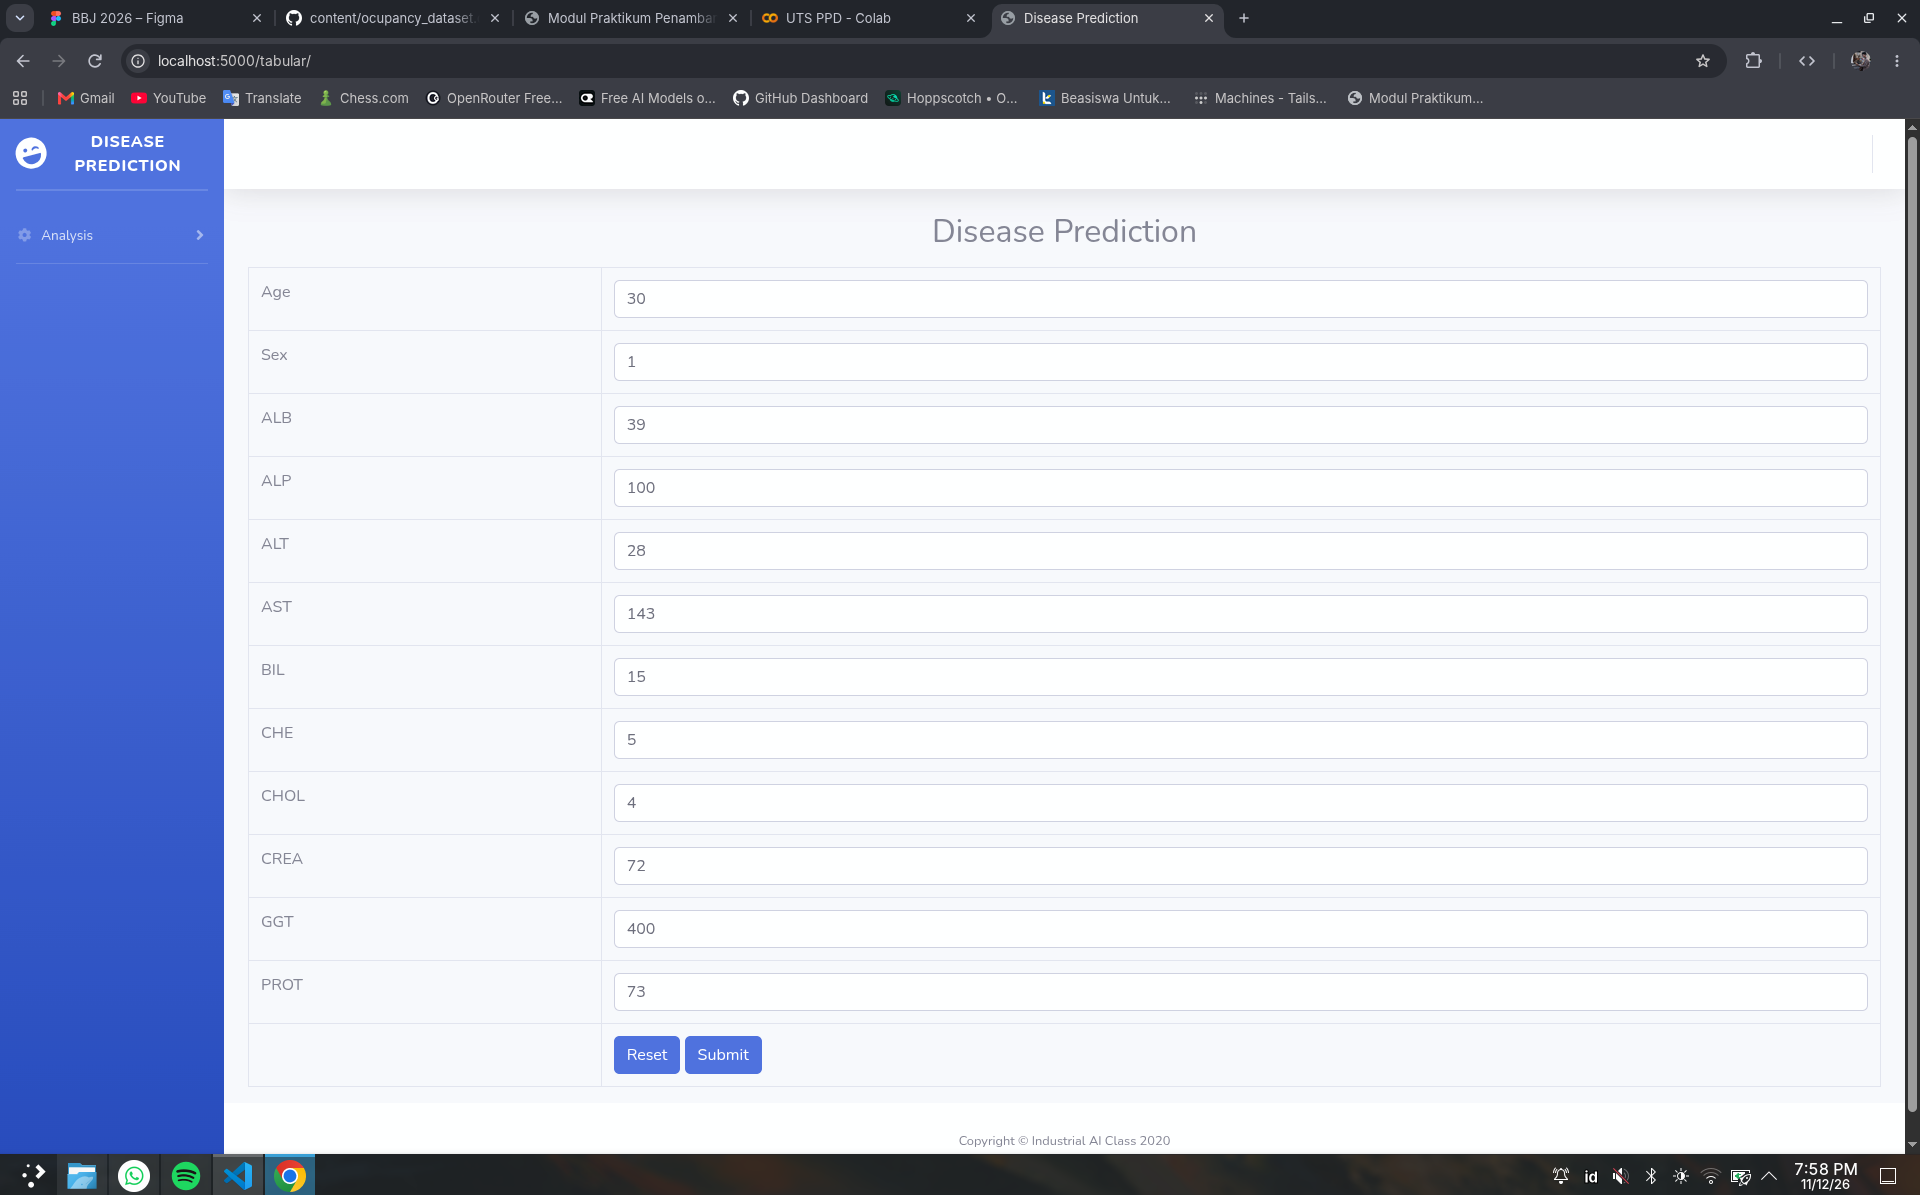
\includegraphics[width=0.8\textwidth]{resource/dokumentasi/1-form-input-tabular-hcv.png}
  \caption{Visualisasi Antarmuka Formulir Input \textit{Disease Prediction} pada Endpoint \texttt{/tabular/}}
  \label{fig:form-input-tabular-hcv-1}
\end{figure}

\par Sebagaimana ditampilkan pada Gambar \ref{fig:form-input-tabular-hcv-1}, akses melalui peramban web ke alamat \url{http://localhost:5000/tabular/} menyajikan halaman antarmuka \textit{Disease Prediction} berbasis templat Bootstrap SB Admin 2. Halaman ini memuat tabel formulir input dua belas parameter biokimia darah dan demografi pasien mulai dari \texttt{Age} hingga \texttt{PROT} yang telah diisi dengan nilai uji standar modul, dilengkapi tombol aksi \texttt{Reset} untuk mengembalikan nilai awal dan tombol \texttt{Submit} untuk mengirimkan data secara \texttt{POST} menuju rute inferensi \texttt{/tabular/result/}.

\begin{figure}[H]
  \centering
  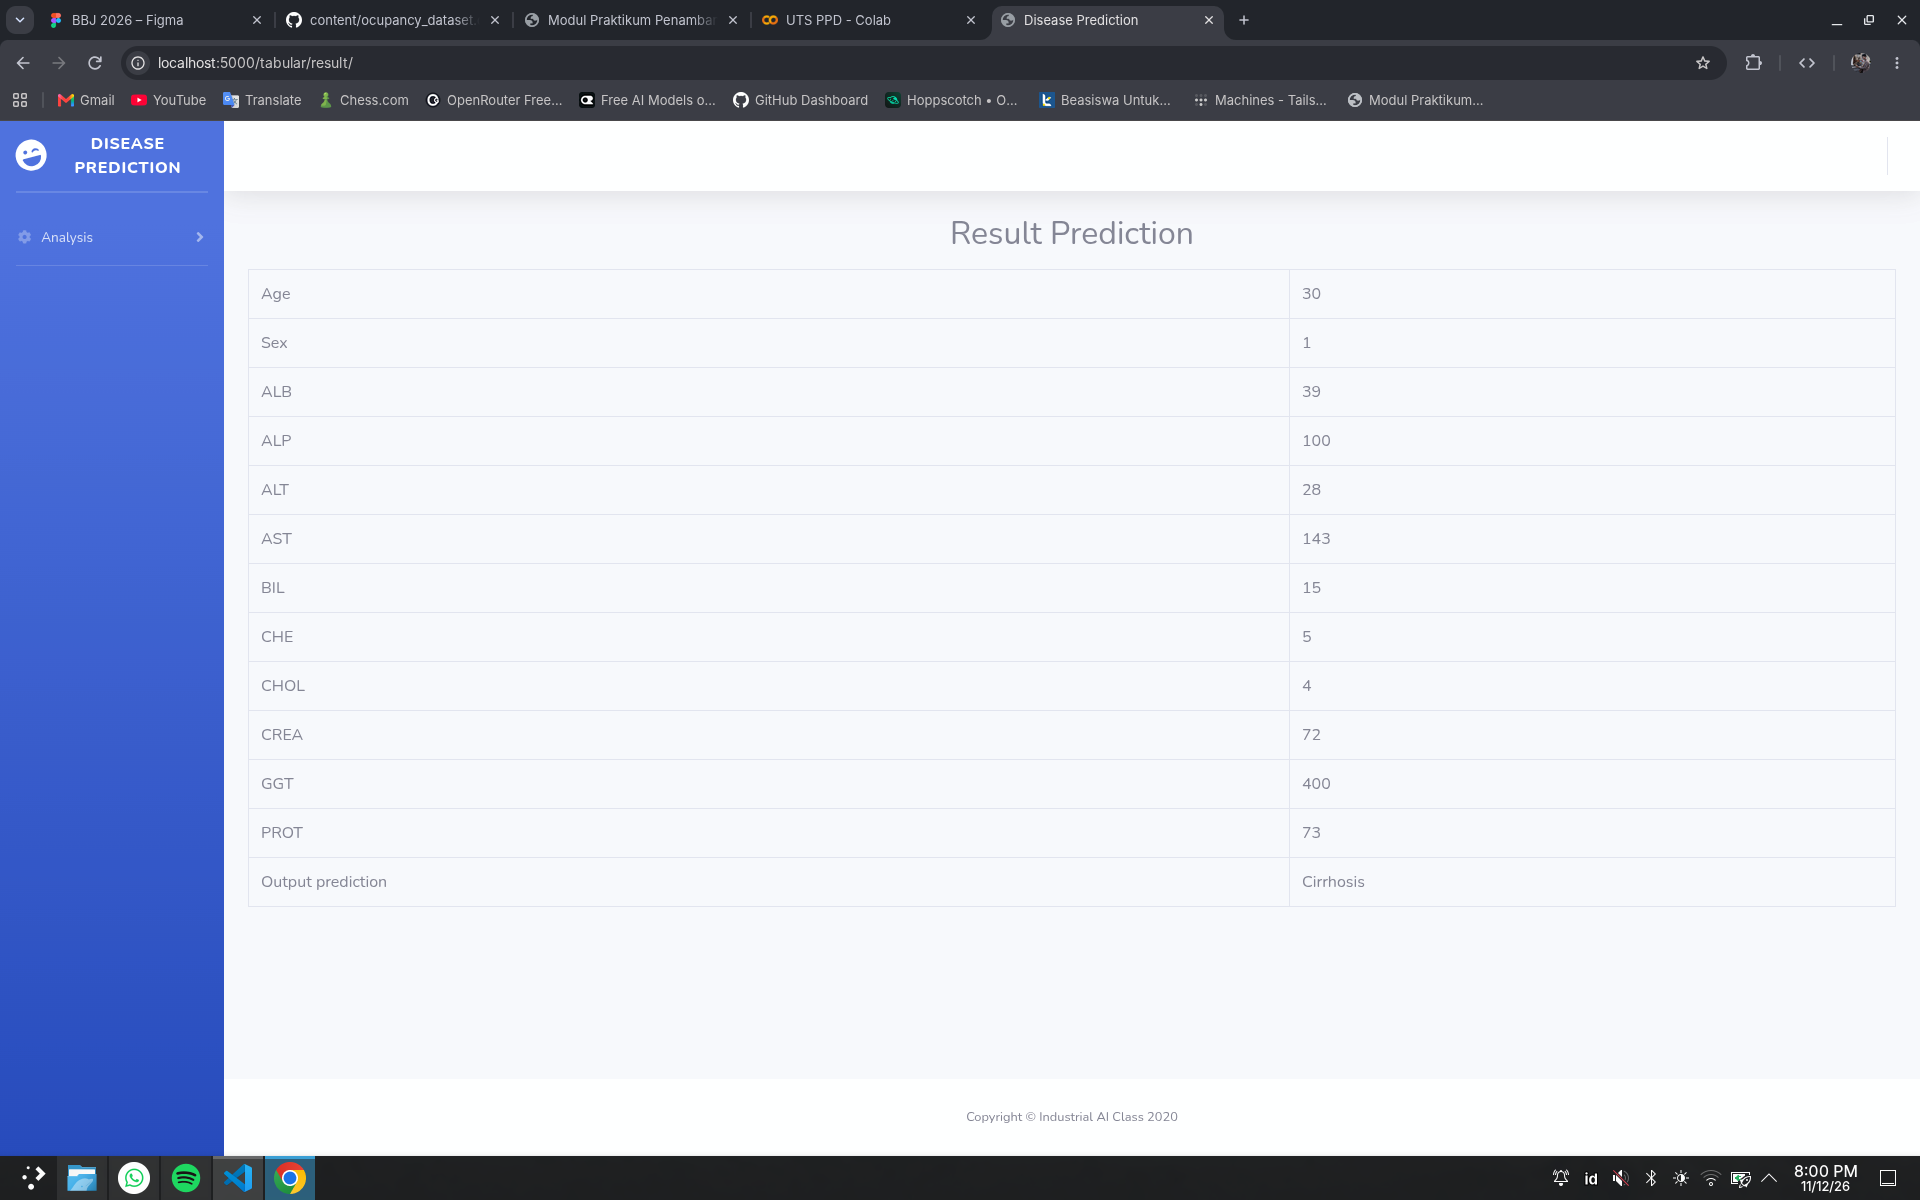
\includegraphics[width=0.8\textwidth]{resource/dokumentasi/2-hasil-prediksi-tabular-hcv.png}
  \caption{Visualisasi Halaman \textit{Result Prediction} pada Endpoint \texttt{/tabular/result/}}
  \label{fig:hasil-prediksi-tabular-hcv-2}
\end{figure}

\par Lebih lanjut pada Gambar \ref{fig:hasil-prediksi-tabular-hcv-2}, setelah tombol \texttt{Submit} ditekan, aplikasi Flask merender halaman \textit{Result Prediction} pada alamat \url{http://localhost:5000/tabular/result/}. Tabel hasil tersebut menampilkan kembali rincian kedua belas nilai parameter yang dimasukkan oleh pengguna beserta baris kesimpulan paling bawah \texttt{Output prediction} yang bernilai \texttt{Cirrhosis}. Tingginya nilai enzim hati \texttt{AST} ($143$) dan \texttt{GGT} ($400$) pada sampel uji tersebut dikenali oleh cabang keputusan model \texttt{DecisionTreeClassifier} sebagai indikator klinis kelas ke-$3$ (\texttt{Cirrhosis}), yang membuktikan bahwa integrasi antara formulir HTML, pemrosesan fitur di Flask, dan deserialisasi model telah bekerja secara akurat.


\subsection{Tugas \& Analisis}
\textbf{Soal:} Silakan menggunakan dataset dari proyek kelompok untuk melakukan pelatihan model, kemudian buatlah \textit{dashboard} dengan Flask. Setelah itu, buatlah laporan praktikumnya.

\subsubsection{Eksplorasi Dataset, Pelatihan Komparatif Lima Model, dan Serialisasi Pipeline}
\lstinputlisting[language=Python, caption={Pelatihan Komparatif Lima Model Klasifikasi dan Serialisasi Pipeline Room Occupancy}, label={lst:kode-tugas-train-occupancy-1}]{resource/code/tugas-train-occupancy_1.py}
\par \textbf{Output:}
\lstinputlisting[caption={Output Evaluasi Lima Model Klasifikasi dan Penyimpanan Artefak Room Occupancy}, label={lst:out-tugas-train-occupancy-1}]{resource/output/tugas-train-occupancy_1_out.txt}
\par \textbf{Analisis:} Berdasarkan penyelesaian pada Kode \ref{lst:kode-tugas-train-occupancy-1}, pengembangan proyek tugas menggunakan dataset sensor lingkungan ruangan kantor \textit{Room Occupancy Detection} (\path{ocupancy_dataset.csv}) \cite{candanedo2016accurate}. Lima atribut sensor fisik ditetapkan sebagai fitur prediktor (\path{FEATURE_COLUMNS}), yaitu suhu ruangan (\texttt{Temperature} dalam $^\circ\text{C}$), kelembapan relatif (\texttt{Humidity} dalam $\%$), intensitas cahaya (\texttt{Light} dalam \textit{Lux}), kadar karbon dioksida (\texttt{CO2} dalam \textit{ppm}), serta rasio kelembapan (\texttt{HumidityRatio} dalam $\text{kg-water-vapor/kg-air}$), sedangkan atribut \texttt{Occupancy} menjadi target biner (\texttt{0} untuk ruangan kosong dan \texttt{1} untuk ruangan terisi). Dataset dibagi menggunakan skema \textit{train-test split} dengan proporsi $70\%$ data latih dan $30\%$ data uji (\path{test_size=0.3, random_state=8}). Selanjutnya, fungsi \path{evaluate_models()} membungkus masing-masing dari lima kandidat algoritma klasifikasi---yakni Logistic Regression, K-Nearest Neighbors ($k=10$), Decision Tree berkriteria \texttt{entropy}, Random Forest, dan AdaBoost---ke dalam objek \path{Pipeline} yang diawali oleh tahapan standarisasi fitur \path{StandardScaler()}. Mengacu pada hasil eksekusi di Output \ref{lst:out-tugas-train-occupancy-1}, dataset memiliki total $20.560$ baris tanpa \textit{missing values} ($0$) dengan distribusi kelas yang tidak seimbang (\textit{imbalanced}), yakni $15.810$ sampel kelas \texttt{0} ($76{,}90\%$) dan $4.750$ sampel kelas \texttt{1} ($23{,}10\%$), yang terbagi menjadi $14.392$ baris data latih dan $6.168$ baris data uji. Rincian lengkap perbandingan metrik evaluasi kelima model pada \textit{test set} beserta struktur \textit{confusion matrix}-nya dirangkum pada Tabel \ref{tab:evaluasi-occupancy}.

\begin{table}[H]
  \centering
  \renewcommand{\arraystretch}{1.25}
  \resizebox{\textwidth}{!}{%
    \begin{tabular}{|l|c|c|c|c|c|}
      \hline
      \textbf{Model Klasifikasi (dalam \texttt{Pipeline})} & \textbf{\textit{Accuracy}} & \textbf{\textit{Macro Precision}} & \textbf{\textit{Macro Recall}} & \textbf{\textit{Macro F1-Score}} & \textbf{\textit{Confusion Matrix}} \texttt{[[TN, FP], [FN, TP]]} \\ \hline
      Logistic Regression                       & $0{,}9882$ & $0{,}9769$ & $0{,}9908$ & $0{,}9836$ & \texttt{[[4673, 67], [6, 1422]]}   \\ \hline
      KNN ($k=10$)                              & $0{,}9895$ & $0{,}9820$ & $0{,}9887$ & $0{,}9853$ & \texttt{[[4693, 47], [18, 1410]]}  \\ \hline
      \textbf{Decision Tree (\texttt{entropy})} & \textbf{$0{,}9909$} & \textbf{$0{,}9882$} & \textbf{$0{,}9863$} & \textbf{$0{,}9872$} & \textbf{\texttt{[[4716, 24], [32, 1396]]}} \\ \hline
      Random Forest                             & $0{,}9908$ & $0{,}9855$ & $0{,}9886$ & $0{,}9871$ & \texttt{[[4705, 35], [22, 1406]]}  \\ \hline
      AdaBoost                                  & $0{,}9887$ & $0{,}9778$ & $0{,}9911$ & $0{,}9843$ & \texttt{[[4676, 64], [6, 1422]]}   \\ \hline
    \end{tabular}%
  }
  \caption{Perbandingan Kinerja Lima Model Klasifikasi pada \textit{Test Set} Dataset \textit{Room Occupancy}}
  \label{tab:evaluasi-occupancy}
\end{table}

\par \textbf{Analisis Pemilihan Model dan Serialisasi Artefak:} Berdasarkan Tabel \ref{tab:evaluasi-occupancy}, seluruh kandidat model menunjukkan kemampuan klasifikasi yang sangat tinggi di atas $98{,}8\%$ berkat kuatnya daya pisah fitur pencahayaan (\texttt{Light}) dan kadar \texttt{CO2} terhadap keberadaan penghuni ruangan. Di antara kelima kandidat, algoritma \textbf{Decision Tree (\texttt{entropy})} terpilih sebagai model terbaik karena meraih skor \textit{accuracy} tertinggi sebesar $0{,}9909$ ($99{,}09\%$), \textit{macro precision} tertinggi sebesar $0{,}9882$, serta \textit{macro F1-score} tertinggi sebesar $0{,}9872$, dengan total kesalahan prediksi paling sedikit yakni hanya $24 + 32 = 56$ sampel dari $6.168$ data uji. Objek \texttt{Pipeline} terbaik tersebut kemudian diserialisasikan menggunakan \path{joblib.dump()} menjadi berkas \path{occupancy_model.joblib} ($22\text{ KB}$), sedangkan seluruh ringkasan statistik dataset, rentang nilai minimum--rata-rata--maksimum tiap sensor, tabel metrik evaluasi kelima model, serta kasus sampel uji otomatis disimpan ke dalam berkas metadata \path{analysis_summary.json} ($2{,}8\text{ KB}$) di direktori \path{tugas/web/artifacts/} agar dapat dirender secara dinamis oleh \textit{dashboard} Flask.

\subsubsection{Pembangunan Aplikasi Dashboard dan Endpoint Prediksi Flask}
\lstinputlisting[language=Python, caption={Implementasi Aplikasi Dashboard dan Endpoint Prediksi Room Occupancy}, label={lst:kode-tugas-flask-app-1}]{resource/code/tugas-flask-app_1.py}
\par \textbf{Output:}
\lstinputlisting[caption={Output Pengujian Endpoint Dashboard Flask, Inferensi Dua Kelas, dan Validasi Input}, label={lst:out-tugas-flask-app-1}]{resource/output/tugas-flask-app_1_out.txt}
\par \textbf{Analisis:} Berdasarkan penyelesaian pada Kode \ref{lst:kode-tugas-flask-app-1}, aplikasi web Flask untuk proyek tugas dirancang berjalan pada port \texttt{5001} dengan memuat dua artefak utama saat inisialisasi server, yaitu objek \textit{pipeline} \path{occupancy_model.joblib} ke dalam konstanta \path{LOADED_MODEL} dan struktur metadata \path{analysis_summary.json} ke dalam kamus \path{ANALYSIS_SUMMARY}. Berbeda dengan aplikasi latihan yang langsung mengonversi string tanpa penanganan kesalahan, fungsi \path{_parse_features()} pada aplikasi tugas melakukan validasi ketat terhadap kelima bidang input sensor: apabila terdapat kolom yang kosong atau berisi teks non-numerik yang memicu \texttt{ValueError}, fungsi akan mengumpulkan pesan kesalahan dan mengembalikan halaman \textit{dashboard} beserta status \texttt{HTTP 400} (\textit{Bad Request}). Pada rute \path{/predict} (\texttt{POST}), data sensor yang valid dibentuk menjadi \path{pd.DataFrame} sesuai urutan \path{FEATURE_COLUMNS} dan langsung diprediksi oleh \path{LOADED_MODEL.predict(df_input)}. Karena objek yang dimuat adalah \texttt{Pipeline}, tahapan \texttt{StandardScaler} otomatis menstandarisasi kelima nilai sensor sebelum diteruskan ke pohon keputusan. Selain label kelas diskret, aplikasi juga memanggil metode \path{LOADED_MODEL.predict_proba(df_input)} untuk menghitung persentase tingkat keyakinan model (\textit{confidence score}) pada masing-masing kelas. Pengujian otomatis menggunakan \texttt{curl} pada Output \ref{lst:out-tugas-flask-app-1} membuktikan bahwa keempat skenario uji berjalan sempurna: akses \texttt{GET /} mengembalikan \texttt{HTTP 200}, pengiriman sampel ruangan terisi menghasilkan prediksi \texttt{Occupied (Terisi)} dengan \texttt{Confidence: 100.0\%} (\texttt{HTTP 200}), pengiriman sampel ruangan kosong menghasilkan prediksi \texttt{Not Occupied (Kosong)} dengan \texttt{Confidence: 100.0\%} (\texttt{HTTP 200}), serta pengujian injeksi input tidak valid (\texttt{Temperature=abc}) berhasil ditangkal dengan respons \texttt{HTTP 400}.

\subsubsection{Pengujian Antarmuka Dashboard Flask dan Analisis Komparatif Deployment}

\begin{figure}[H]
  \centering
  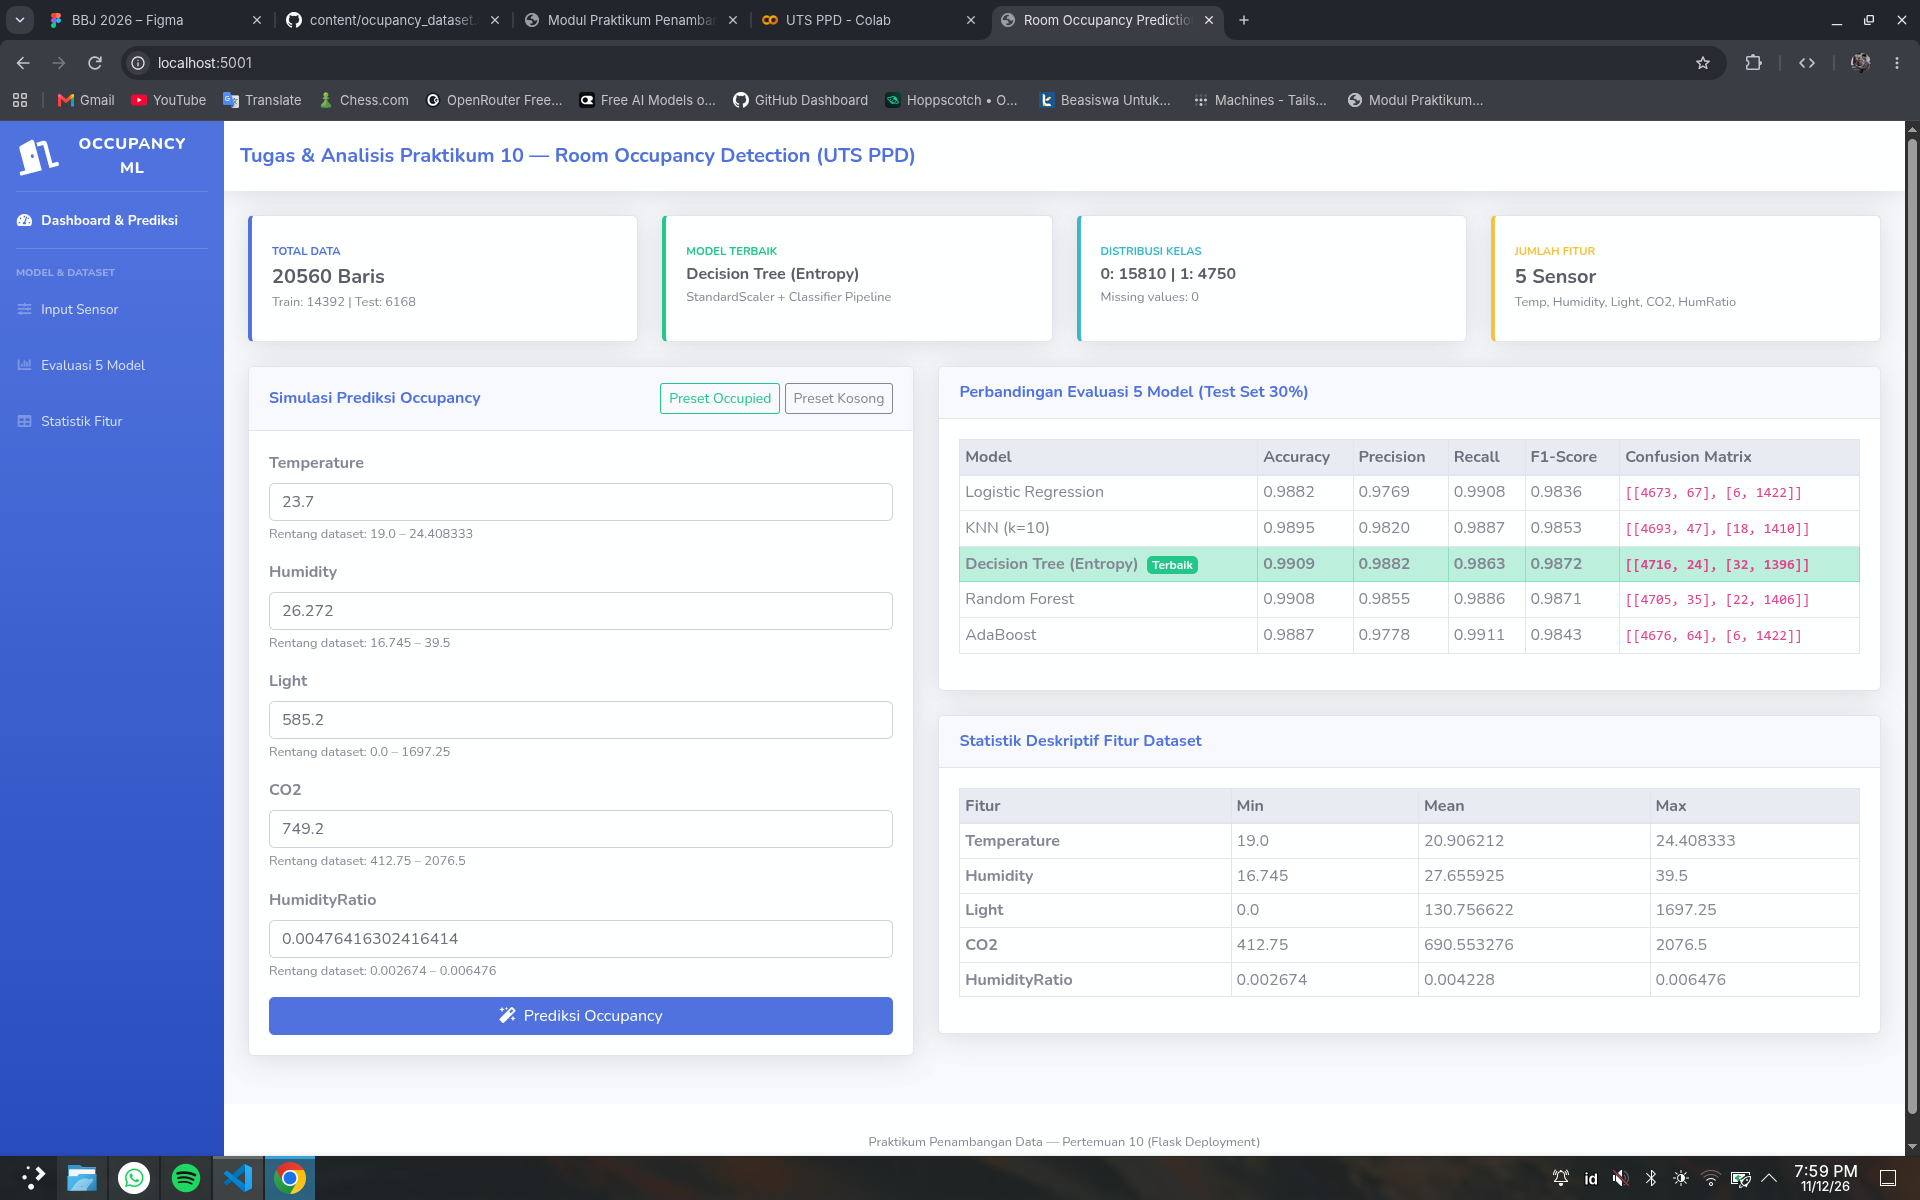
\includegraphics[width=0.8\textwidth]{resource/dokumentasi/tugas-1-dashboard-occupancy-flask.png}
  \caption{Visualisasi Halaman Utama \textit{Dashboard} Flask \textit{Room Occupancy Detection} pada \texttt{http://localhost:5001}}
  \label{fig:tugas-dashboard-occupancy-flask-1}
\end{figure}

\par \textbf{Analisis:} Sebagaimana ditampilkan pada Gambar \ref{fig:tugas-dashboard-occupancy-flask-1}, antarmuka utama \textit{dashboard} Flask di alamat \url{http://localhost:5001} menyajikan pusat informasi analitik dan simulasi prediksi secara terpadu dalam satu layar. Pada baris teratas terdapat empat kartu ringkasan metrik utama yang memuat informasi \texttt{Total Data} ($20.560$ baris; \path{Train: 14392 | Test: 6168}), \texttt{Model Terbaik} (\path{Decision Tree (Entropy)} dalam komposisi \path{StandardScaler + Classifier}), \texttt{Distribusi Kelas} (\path{0: 15810 | 1: 4750} dengan \path{Missing values: 0}), serta \texttt{Jumlah Fitur} ($5$ sensor). Pada kolom kiri tersedia panel \textit{Simulasi Prediksi Occupancy} yang dilengkapi dua tombol pengisian cepat berbasis JavaScript (\texttt{Preset Occupied} dan \texttt{Preset Kosong}) beserta panduan rentang nilai minimum hingga maksimum dataset di bawah setiap kolom input. Adapun pada kolom kanan disajikan tabel \textit{Perbandingan Evaluasi 5 Model (Test Set 30\%)} dengan penanda baris hijau pada model terbaik serta tabel \textit{Statistik Deskriptif Fitur Dataset} yang menampilkan nilai \texttt{Min}, \texttt{Mean}, dan \texttt{Max} dari kelima sensor.

\begin{figure}[H]
  \centering
  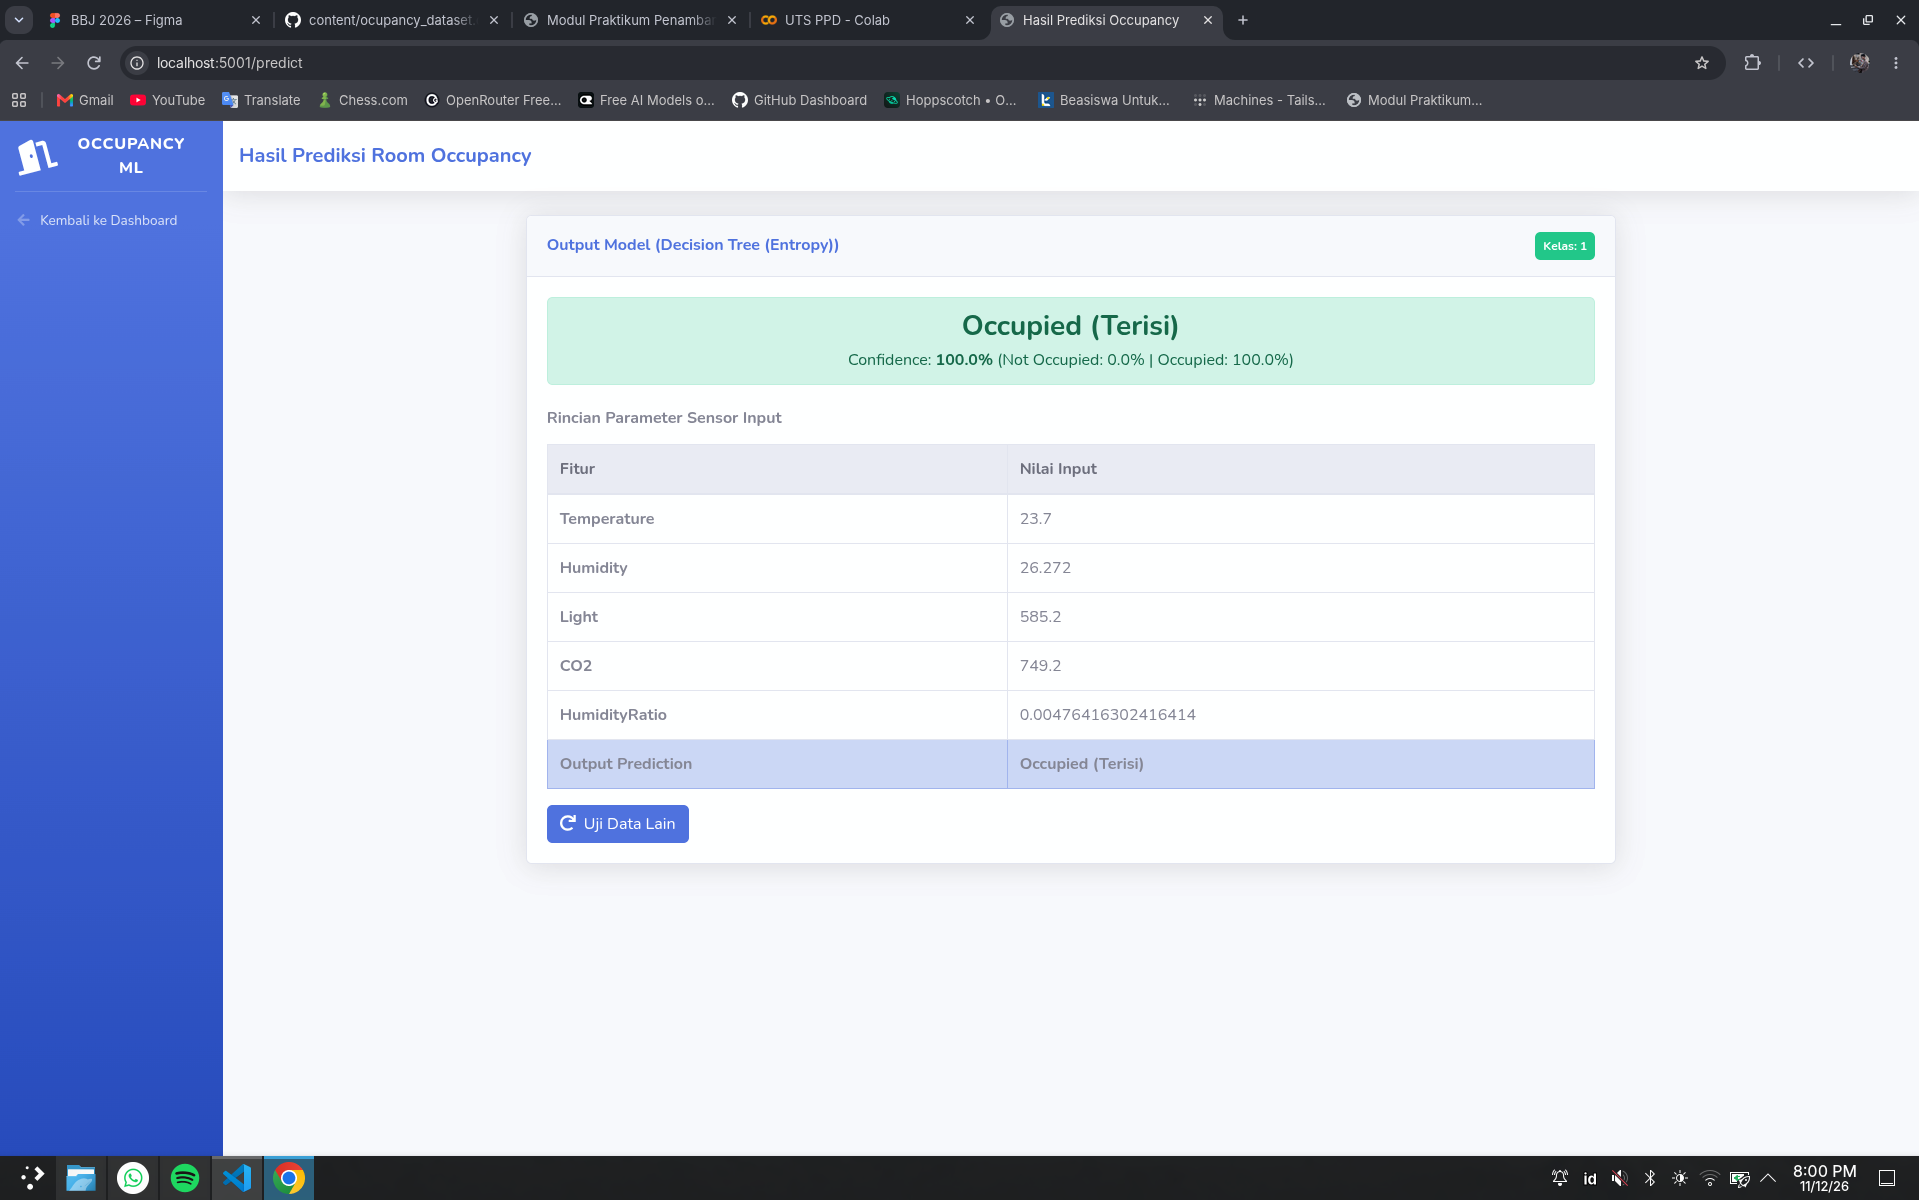
\includegraphics[width=0.8\textwidth]{resource/dokumentasi/tugas-2-hasil-prediksi-occupancy-flask.png}
  \caption{Visualisasi Halaman Hasil Prediksi \textit{Room Occupancy} pada Endpoint \texttt{/predict}}
  \label{fig:tugas-hasil-prediksi-occupancy-flask-2}
\end{figure}

\par \textbf{Analisis:} Lebih lanjut pada Gambar \ref{fig:tugas-hasil-prediksi-occupancy-flask-2}, ketika pengguna menekan tombol \texttt{Prediksi Occupancy} dengan nilai sensor \path{Temperature = 23.7}, \path{Humidity = 26.272}, \path{Light = 585.2}, \path{CO2 = 749.2}, serta \path{HumidityRatio = 0.00476416302416414}, aplikasi mengarahkan tampilan menuju halaman \url{http://localhost:5001/predict}. Halaman ini menampilkan kotak status berwarna hijau dengan keputusan \textbf{\texttt{Occupied (Terisi)}} (\texttt{Kelas: 1}) beserta rincian probabilitas \path{Confidence: 100.0% (Not Occupied: 0.0% | Occupied: 100.0%)}, tabel rekapitulasi nilai parameter sensor yang diinputkan, serta tombol navigasi \texttt{Uji Data Lain} untuk kembali ke halaman \textit{dashboard}.

\par Guna memberikan gambaran menyeluruh mengenai peningkatan kualitas rekayasa perangkat lunak dan arsitektur \textit{deployment} yang diterapkan dari proyek latihan menuju proyek tugas, perbandingan spesifikasi teknis kedua sistem dirangkum pada Tabel \ref{tab:komparasi-deployment}.

\begin{table}[H]
  \centering
  \renewcommand{\arraystretch}{1.25}
  \resizebox{\textwidth}{!}{%
    \begin{tabular}{|l|p{6.2cm}|p{6.5cm}|}
      \hline
      \textbf{Aspek Arsitektur \& Teknis} & \textbf{Proyek Latihan (\textit{Hepatitis C Prediction})} & \textbf{Proyek Tugas (\textit{Room Occupancy Dashboard})} \\ \hline
      Dataset \& Skala Sampel & \texttt{hcvdat0.csv} ($615 \rightarrow 589$ baris bersih, $12$ fitur klinis, $4$ kelas target) & \texttt{ocupancy\_dataset.csv} ($20.560$ baris bersih, $5$ fitur sensor lingkungan, $2$ kelas target) \\ \hline
      Strategi Pelatihan \& Evaluasi & Pelatihan tunggal \texttt{DecisionTreeClassifier} pada seluruh data (\textit{in-sample accuracy} $1{,}0000$) & Evaluasi komparatif $5$ algoritma dengan \textit{train-test split} $70:30$ (\textit{test accuracy} terbaik $0{,}9909$) \\ \hline
      Objek yang Diserialisasikan & Estimator \texttt{DecisionTreeClassifier} mandiri (\texttt{dt\_model.model}, $5{,}7\text{ KB}$) & Komposisi \texttt{Pipeline(StandardScaler + DecisionTreeClassifier)} (\texttt{occupancy\_model.joblib}, $22\text{ KB}$) \\ \hline
      Artefak Metadata Analitik & Tidak ada (hanya memuat berkas model biner) & Menyertakan \texttt{analysis\_summary.json} ($2{,}8\text{ KB}$) berisi metrik $5$ model, statistik fitur, dan sampel uji \\ \hline
      Penanganan \textit{Preprocessing} Saat Inferensi & Konversi manual melalui fungsi \texttt{\_encode\_sex()} dan \texttt{\_to\_float()} di dalam \textit{route} Flask & Validasi numerik ketat \texttt{\_parse\_features()} + penskalaan otomatis oleh \texttt{StandardScaler} di dalam \texttt{Pipeline} \\ \hline
      Validasi Kesalahan Input Pengguna & Input kosong diubah menjadi \texttt{NaN}; belum mengembalikan kode galat HTTP khusus & Menolak input kosong atau teks non-numerik dengan pesan peringatan UI dan status \texttt{HTTP 400} \\ \hline
      Informasi Keluaran Inferensi & Hanya menampilkan nama kelas hasil \texttt{predict()} pada tabel HTML & Menampilkan label kelas, lencana indeks kelas, serta persentase \textit{confidence} dari \texttt{predict\_proba()} \\ \hline
      Port \& Endpoint Layanan Flask & Port \texttt{5000}: \texttt{GET /tabular/} dan \texttt{POST /tabular/result/} & Port \texttt{5001}: \texttt{GET /} (\textit{Dashboard}) dan \texttt{POST /predict} \\ \hline
    \end{tabular}%
  }
  \caption{Perbandingan Arsitektur dan Spesifikasi Teknis \textit{Model Deployment} antara Proyek Latihan dan Proyek Tugas}
  \label{tab:komparasi-deployment}
\end{table}

\par \textbf{Analisis Komparatif:} Mengacu pada Tabel \ref{tab:komparasi-deployment}, pengembangan pada proyek tugas menerapkan tiga praktik rekayasa \textit{deployment} yang jauh lebih matang dibandingkan proyek latihan dasar. Pertama, pembungkusan tahapan \texttt{StandardScaler} bersama model klasifikasi ke dalam satu objek \texttt{Pipeline} sebelum diekspor menggunakan \texttt{joblib.dump()} menghilangkan risiko ketidaksinkronan skala fitur saat inferensi di aplikasi Flask. Kedua, pemisahan hasil evaluasi eksperimen ke dalam artefak JSON (\texttt{analysis\_summary.json}) memungkinkan pembuatan antarmuka \textit{dashboard} yang tidak sekadar menampilkan formulir input kosong, melainkan juga menyajikan transparansi performa kelima model kandidat, rentang nilai wajar setiap sensor, serta tombol pengisian sampel otomatis (\textit{preset}) yang memudahkan pengujian pengguna. Ketiga, penambahan validasi tipe data masukan dengan kode respons \texttt{HTTP 400} serta penyajian skor probabilitas \texttt{predict\_proba()} meningkatkan keandalan layanan web dan memberikan tingkat keterjelasan keputusan (\textit{explainability}) yang lebih baik bagi pengguna akhir.

\subsection{Implementasi Model Deployment Prediksi Penyakit Hepatitis C dengan Streamlit}

\par Pada materi pertemuan ke-11, arsitektur \textit{model deployment} dieksplorasi menggunakan pendekatan \textit{data application framework} berbasis Streamlit. Berbeda dengan Flask yang memisahkan kode logika rute HTTP (\texttt{app.py}) dan templat antarmuka (\texttt{index.html} serta \texttt{result.html}), Streamlit mengadopsi paradigma deklaratif di mana tata letak antarmuka (\textit{user interface}), penerimaan input pengguna, dan eksekusi inferensi model machine learning disatukan secara elegan dalam satu naskah Python murni. Model yang digunakan pada proyek latihan ini adalah estimator \texttt{DecisionTreeClassifier} yang telah dilatih pada dataset Hepatitis C (\path{hcvdat0.csv}) dan disimpan dalam artefak biner \path{dt_model.model}.

\subsubsection{Konfigurasi Antarmuka, Manajemen State, dan Integrasi Model Streamlit}
\lstinputlisting[language=Python, caption={Implementasi Aplikasi Web Prediksi Hepatitis C Berbasis Streamlit}, label={lst:kode-latihan-streamlit-app-1}]{resource/code/latihan-streamlit-app_1.py}
\par \textbf{Output:}
\lstinputlisting[caption={Output Pengujian Layanan dan Verifikasi Endpoint Streamlit Latihan}, label={lst:out-latihan-streamlit-app-1}]{resource/output/latihan-streamlit-app_1_out.txt}
\par \textbf{Analisis:} Berdasarkan implementasi pada Kode \ref{lst:kode-latihan-streamlit-app-1}, aplikasi Streamlit latihan dibangun dengan konfigurasi halaman penuh melalui \path{st.set_page_config(page_title="HCV Predictor", layout="wide")}. Pemuatan model serialisasi dilakukan melalui fungsi pembungkus \path{load_model()} yang dihiasi dekorator \path{@st.cache_resource}. Penggunaan dekorator ini memastikan bahwa artefak \path{dt_model.model} hanya dibaca satu kali dari disk ke dalam memori global pada saat aplikasi pertama kali dinyalakan, sehingga siklus \textit{script rerun} tidak membebani komputasi \textit{I/O}. Antarmuka masukan disusun secara ergonomis menjadi tiga kolom sejajar (\path{st.columns(3)}) menggunakan widget \path{st.number_input()} dan \path{st.selectbox()} untuk atribut kategorikal jenis kelamin (\texttt{Category: Sex}). Nilai teks \texttt{m} atau \texttt{f} dipetakan secara deterministik menjadi representasi numerik biner ($0$ atau $1$) agar selaras dengan skema pelatihan. Ketika pengguna menekan tombol \path{st.button("Prediksi Hasil")}, Streamlit mengeksekusi inferensi \path{model.predict(input_df)} dan menampilkan hasil diagnosis klinis dalam kotak notifikasi berwarna (\path{st.success()}) beserta ringkasan parameter masukan dalam format tabel interaktif (\path{st.dataframe()}). Pada pengujian Output \ref{lst:out-latihan-streamlit-app-1}, verifikasi jaringan berbasis \texttt{curl} ke \url{http://localhost:8501} mengonfirmasi respons \texttt{HTTP/1.1 200 OK} dengan penyisipan berkas statis dan skrip runtime Streamlit secara sempurna.

\subsubsection{Pengujian Antarmuka Aplikasi Streamlit Prediksi Hepatitis C}

\begin{figure}[H]
  \centering
  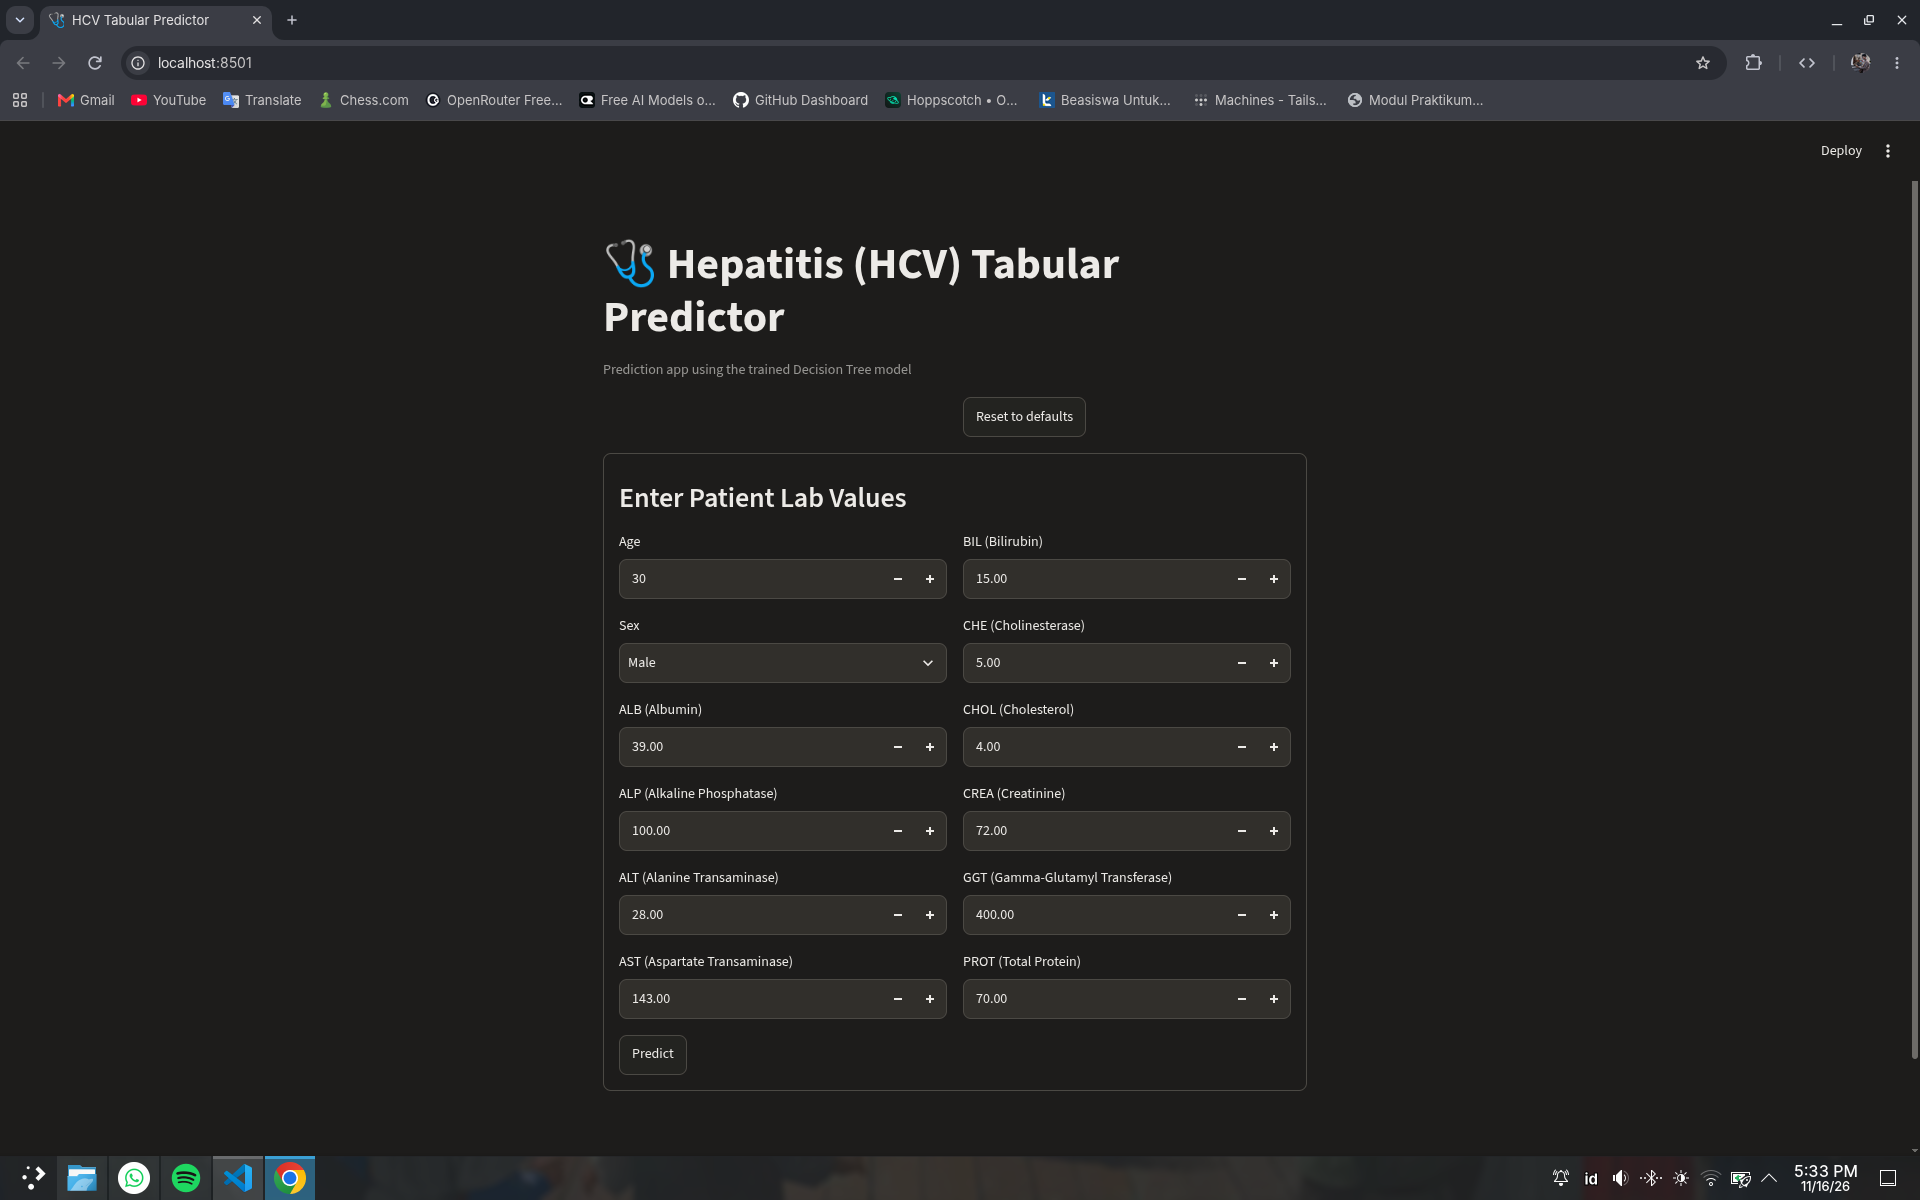
\includegraphics[width=0.8\textwidth]{resource/dokumentasi/1-form-input-tabular-hcv-streamlit.png}
  \caption{Visualisasi Formulir Input Tabular Prediksi Hepatitis C Berbasis Streamlit pada \texttt{http://localhost:8501}}
  \label{fig:latihan-form-input-hcv-streamlit}
\end{figure}

\par \textbf{Analisis:} Gambar \ref{fig:latihan-form-input-hcv-streamlit} memperlihatkan antarmuka web aplikasi prediksi Hepatitis C yang berhasil di-deploy pada port \texttt{8501}. Streamlit secara otomatis merender komponen masukan ke dalam tiga kolom responsif: kolom pertama memuat data demografis (\textit{Age} dan \textit{Sex}) serta enzim hati dasar (\textit{ALB} dan \textit{ALP}), kolom kedua memuat indikator bilirubin dan protein (\textit{ALT}, \textit{AST}, \textit{BIL}, dan \textit{CHE}), sedangkan kolom ketiga memuat parameter kolesterol dan jaringan (\textit{CHOL}, \textit{CREA}, \textit{GGT}, dan \textit{PROT}). Nilai bawaan (\textit{default}) pada setiap kotak input diatur mendekati distribusi sampel uji klinis (\textit{Cirrhosis}) guna memudahkan pengujian tanpa memerlukan penulisan berkas HTML terpisah.

\begin{figure}[H]
  \centering
  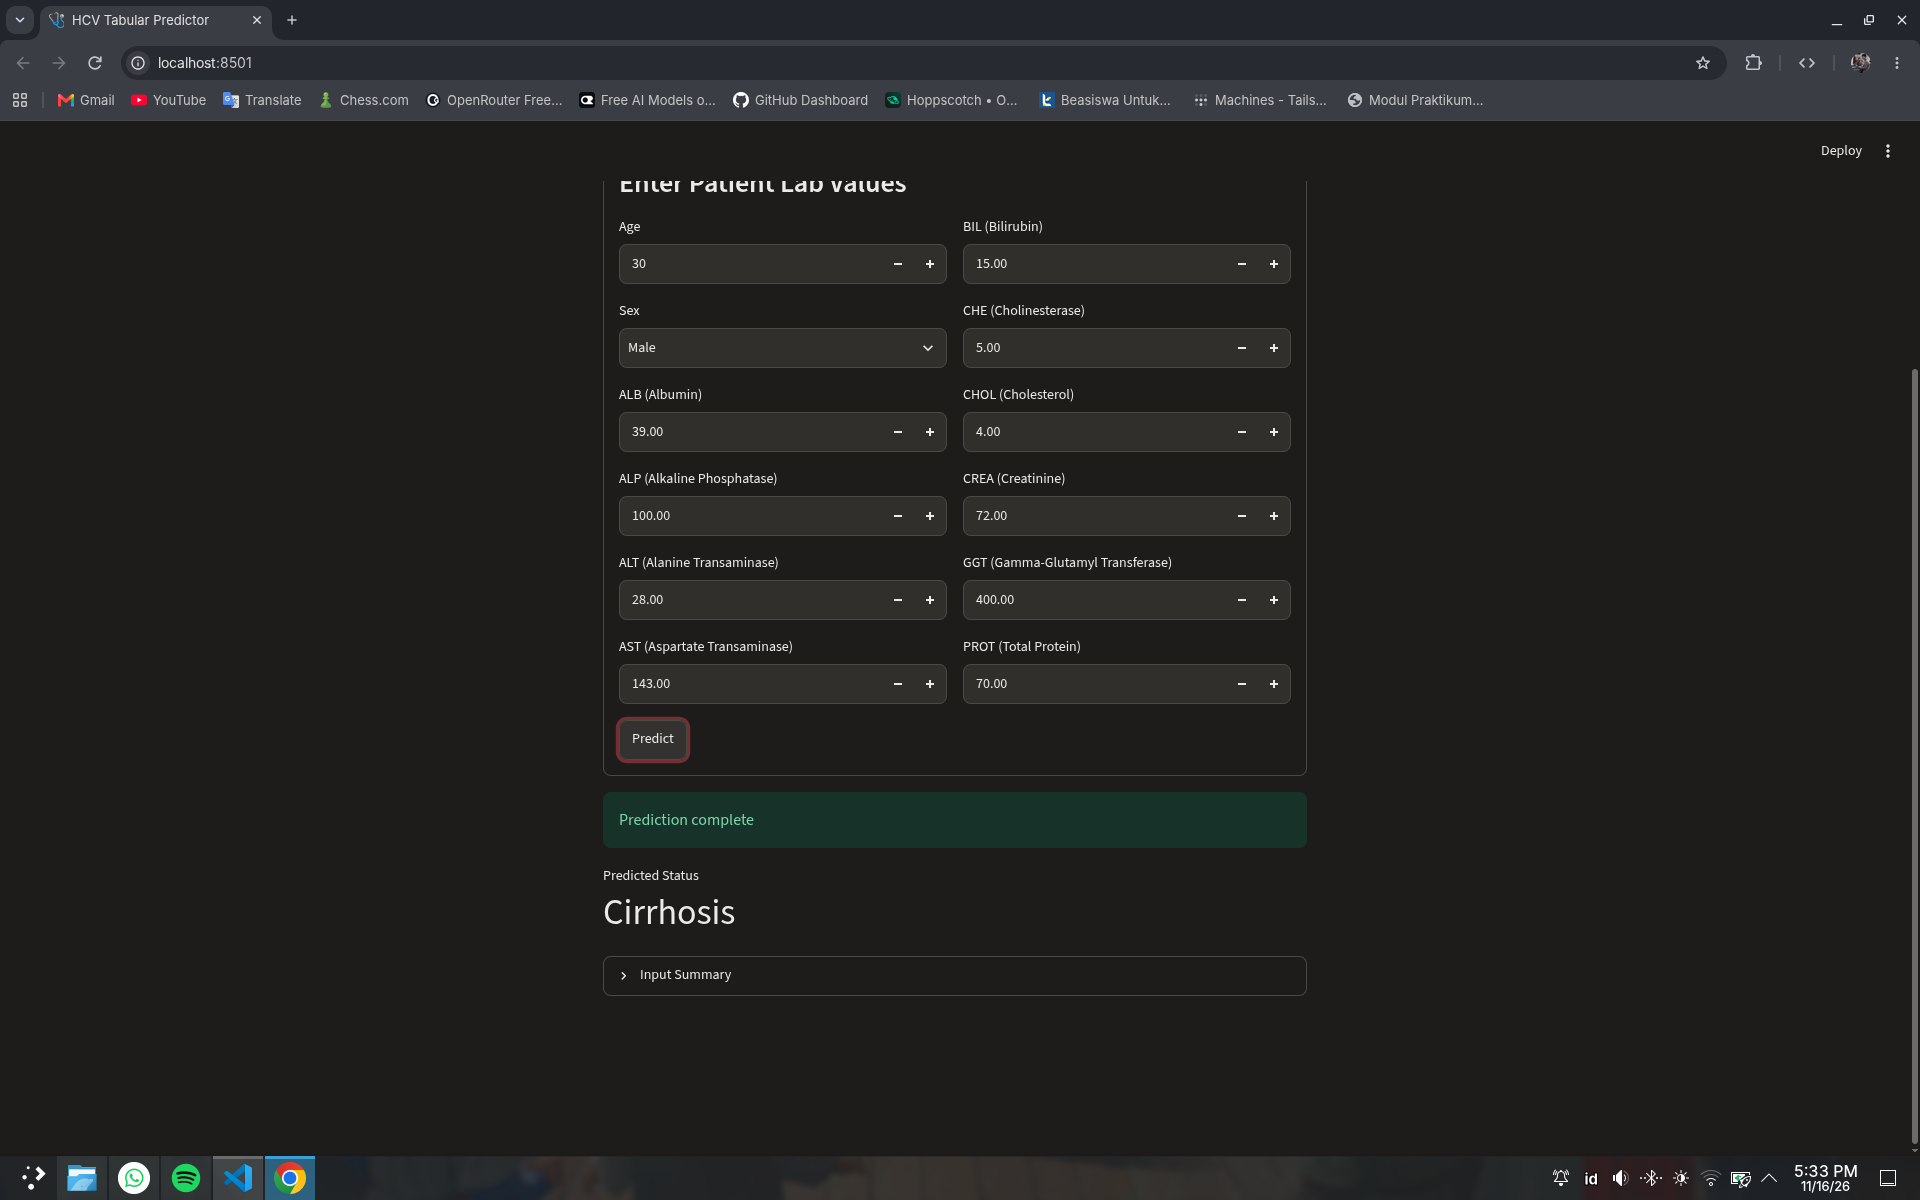
\includegraphics[width=0.8\textwidth]{resource/dokumentasi/2-hasil-prediksi-tabular-hcv-streamlit.png}
  \caption{Visualisasi Hasil Prediksi Klinis Hepatitis C pada Antarmuka Reaktif Streamlit}
  \label{fig:latihan-hasil-prediksi-hcv-streamlit}
\end{figure}

\par \textbf{Analisis:} Ketika tombol \texttt{Prediksi Hasil} ditekan, mekanisme reaktif Streamlit langsung merender bagian visualisasi hasil inferensi tepat di bawah formulir masukan tanpa melakukan \textit{refresh} seluruh halaman peramban, seperti diperlihatkan pada Gambar \ref{fig:latihan-hasil-prediksi-hcv-streamlit}. Aplikasi menampilkan spanduk hijau \path{st.success} yang mengumumkan diagnosis \textbf{\texttt{Hasil Prediksi: Cirrhosis}} disertai visualisasi tabel \textit{dataframe} ringkasan seluruh variabel yang dikirimkan. Hal ini membuktikan bahwa integrasi model serialisasi Scikit-Learn ke dalam lingkungan Streamlit berhasil berjalan secara instan dan interaktif.

\subsection{Tugas \& Analisis 2: Pembangunan Dashboard Interaktif Room Occupancy dengan Streamlit}

\par \textbf{Soal:} Lakukan pembangunan aplikasi data interaktif (\textit{interactive data dashboard}) untuk deteksi keterisian ruangan (\textit{Room Occupancy Detection}) berbasis Streamlit dengan memanfaatkan dataset lingkungan \path{ocupancy_dataset.csv} ($20.560$ baris, $5$ parameter sensor). Sistem wajib memanfaatkan artefak terbaik \path{Pipeline(StandardScaler + DecisionTreeClassifier)} dan metadata eksperimen \path{analysis_summary.json}, menyediakan antarmuka terstruktur berbasis multi-tab, mengimplementasikan mekanisme \textit{preset} skenario (\textit{Occupied} dan \textit{Not Occupied}) melalui manajemen \path{st.session_state}, serta memvisualisasikan estimasi probabilitas kepastian (\textit{confidence score}) dan perbandingan masukan terhadap statistik dataset.

\subsubsection{Arsitektur Dashboard Multi-Tab dan Pengelolaan State Sensor Streamlit}
\lstinputlisting[language=Python, caption={Implementasi Dashboard Interaktif Multi-Tab Room Occupancy Berbasis Streamlit}, label={lst:kode-tugas-streamlit-app-1}]{resource/code/tugas-streamlit-app_1.py}
\par \textbf{Output:}
\lstinputlisting[caption={Output Pengujian Layanan dan Verifikasi Endpoint Streamlit Dashboard Tugas}, label={lst:out-tugas-streamlit-app-1}]{resource/output/tugas-streamlit-app_1_out.txt}
\par \textbf{Analisis:} Kode \ref{lst:kode-tugas-streamlit-app-1} menyajikan implementasi arsitektur \textit{dashboard} analitik modern pada berkas \path{app.py} proyek tugas Streamlit. Aplikasi memanfaatkan dua jenis \textit{caching} Scikit-Learn dan data: \path{@st.cache_resource} untuk memuat objek pipeline \path{occupancy_model.joblib} dan \path{@st.cache_data} untuk memuat metadata \path{analysis_summary.json}. Untuk mengatasi tantangan persistensi data masukan antar-siklus eksekusi, aplikasi menginisialisasi kamus \path{st.session_state} dengan nilai bawaan sensor. Tombol pengisian cepat (\textit{preset}) \texttt{Preset Ruangan Terisi (Occupied)} dan \texttt{Preset Ruangan Kosong (Not Occupied)} menginjeksikan nilai sensor sampel ke dalam \path{st.session_state} dan langsung memicu pembaruan widget \path{st.number_input}. Struktur antarmuka diorganisasikan ke dalam dua tab utama melalui \path{st.tabs(["Simulasi Prediksi Sensor", "Eksplorasi \& Evaluasi Model"])}. Pada tab simulasi, inferensi dilakukan dengan menghitung kelas prediksi melalui \path{model.predict(input_df)} dan probabilitas melalui \path{model.predict_proba(input_df)}. Status keputusan ditampilkan secara kontras menggunakan kotak \path{st.success} hijau (\texttt{Occupied}) atau \path{st.info} biru (\texttt{Not Occupied}), dilengkapi meteran probabilitas visual \path{st.progress()} dan kartu metrik ringkasan \path{st.metric()}. Sementara itu, tab eksplorasi menyajikan transparansi penuh metrik evaluasi kelima model klasifikasi, distribusi data latih/uji, serta tabel acuan rentang nilai sensor minimum, rata-rata, dan maksimum. Pengujian jaringan pada Output \ref{lst:out-tugas-streamlit-app-1} membuktikan bahwa server Streamlit tugas pada port \texttt{8502} merespons dengan status \texttt{HTTP/1.1 200 OK} dan siap melayani permintaan pengguna.

\subsubsection{Pengujian Visual Antarmuka Dashboard dan Simulasi Prediksi Streamlit}

\begin{figure}[H]
  \centering
  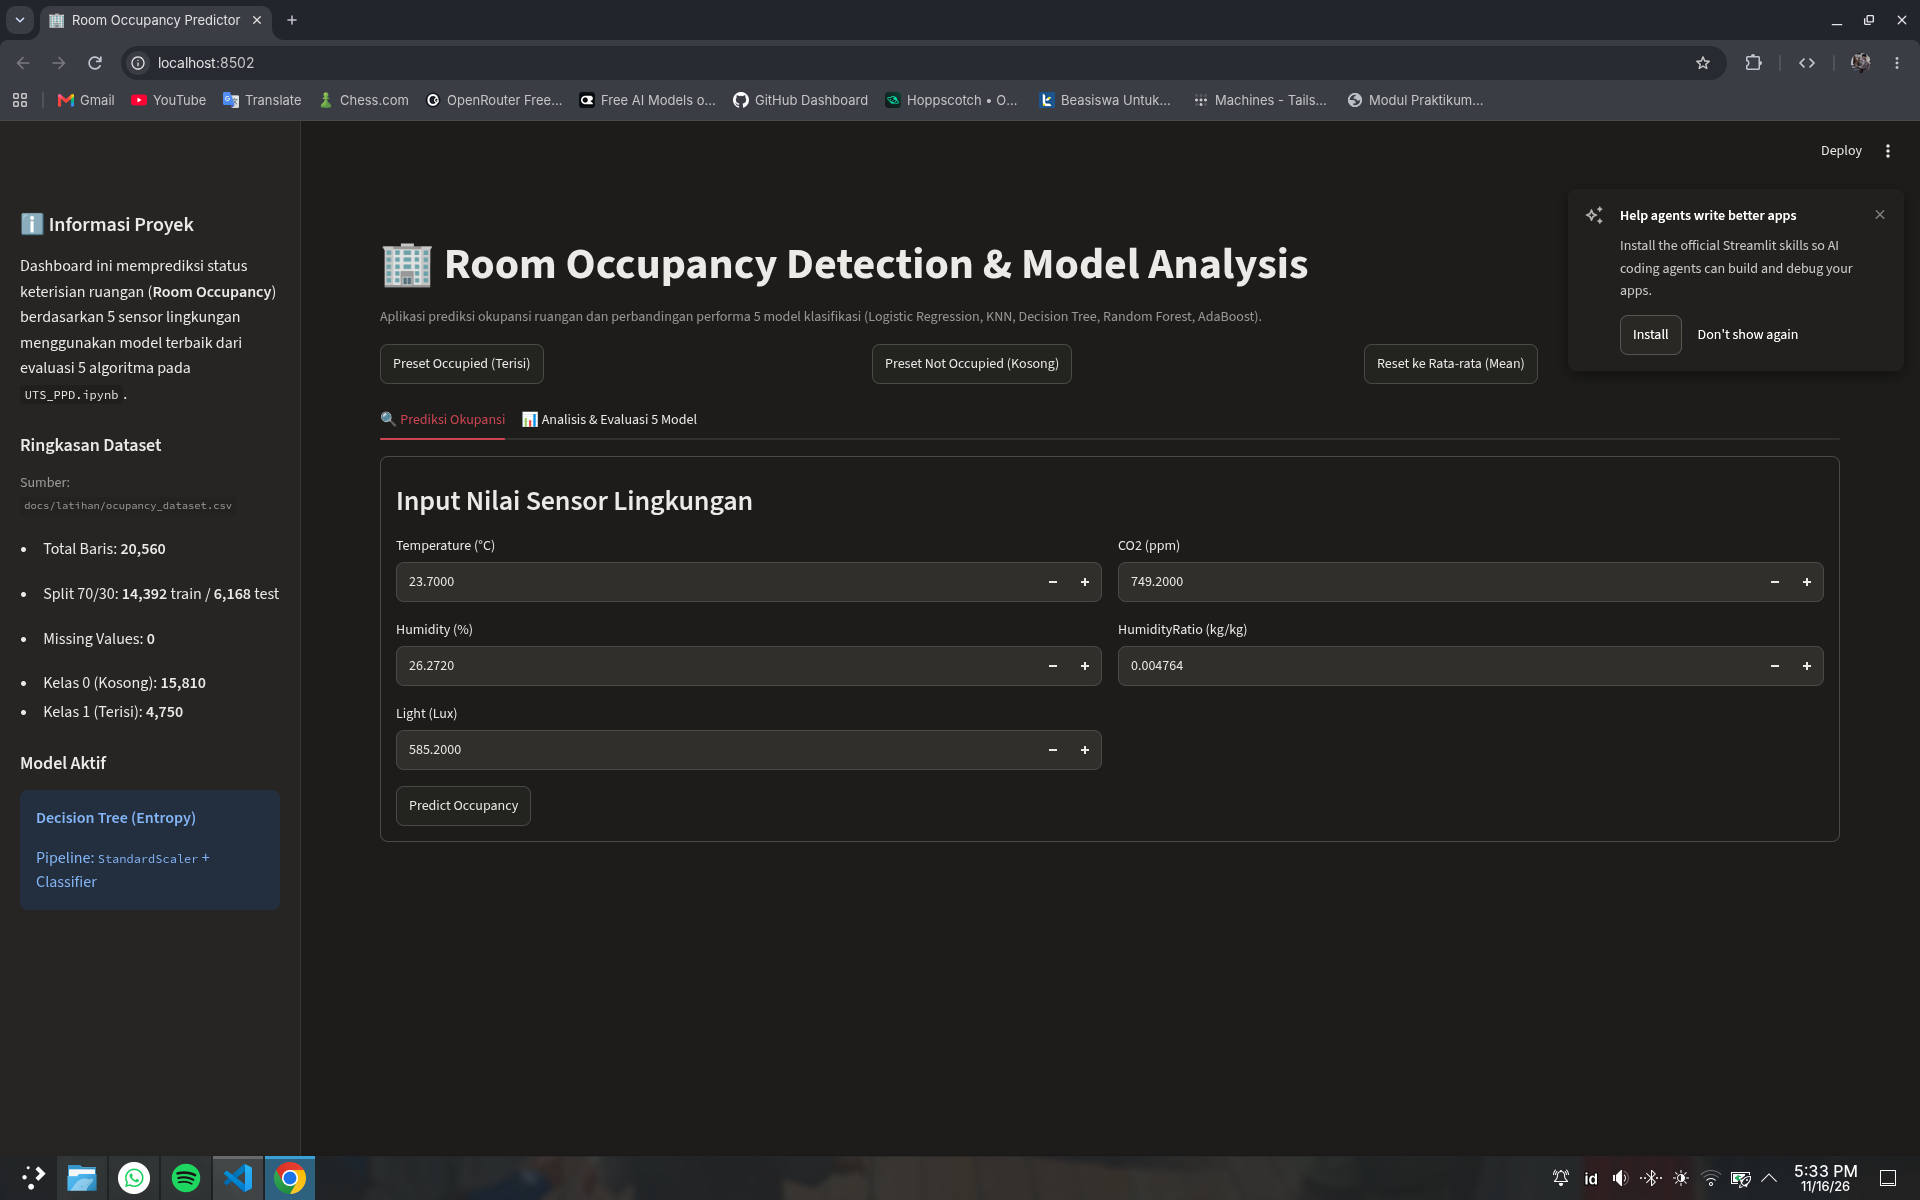
\includegraphics[width=0.8\textwidth]{resource/dokumentasi/tugas-1-dashboard-occupancy-streamlit.png}
  \caption{Visualisasi Tab Simulasi Prediksi dan Panel Preset \textit{Dashboard} Streamlit pada \texttt{http://localhost:8502}}
  \label{fig:tugas-dashboard-occupancy-streamlit-1}
\end{figure}

\par \textbf{Analisis:} Gambar \ref{fig:tugas-dashboard-occupancy-streamlit-1} menunjukkan tampilan awal \textit{dashboard} Streamlit pada port \texttt{8502}. Halaman ini diawali dengan empat kartu metrik informasi dataset ($20.560$ total data, $14.392$ data latih, $6.168$ data uji, dan $5$ sensor lingkungan). Pada Tab \textit{Simulasi Prediksi Sensor}, pengguna disajikan dua tombol aksi pengisian cepat (\textit{Preset Occupied} dan \textit{Preset Kosong}) serta formulir masukan $5$ sensor yang disusun ke dalam dua kolom rapi dengan batasan nilai presisi tinggi sesuai rentang fisikal sensor lingkungan.

\begin{figure}[H]
  \centering
  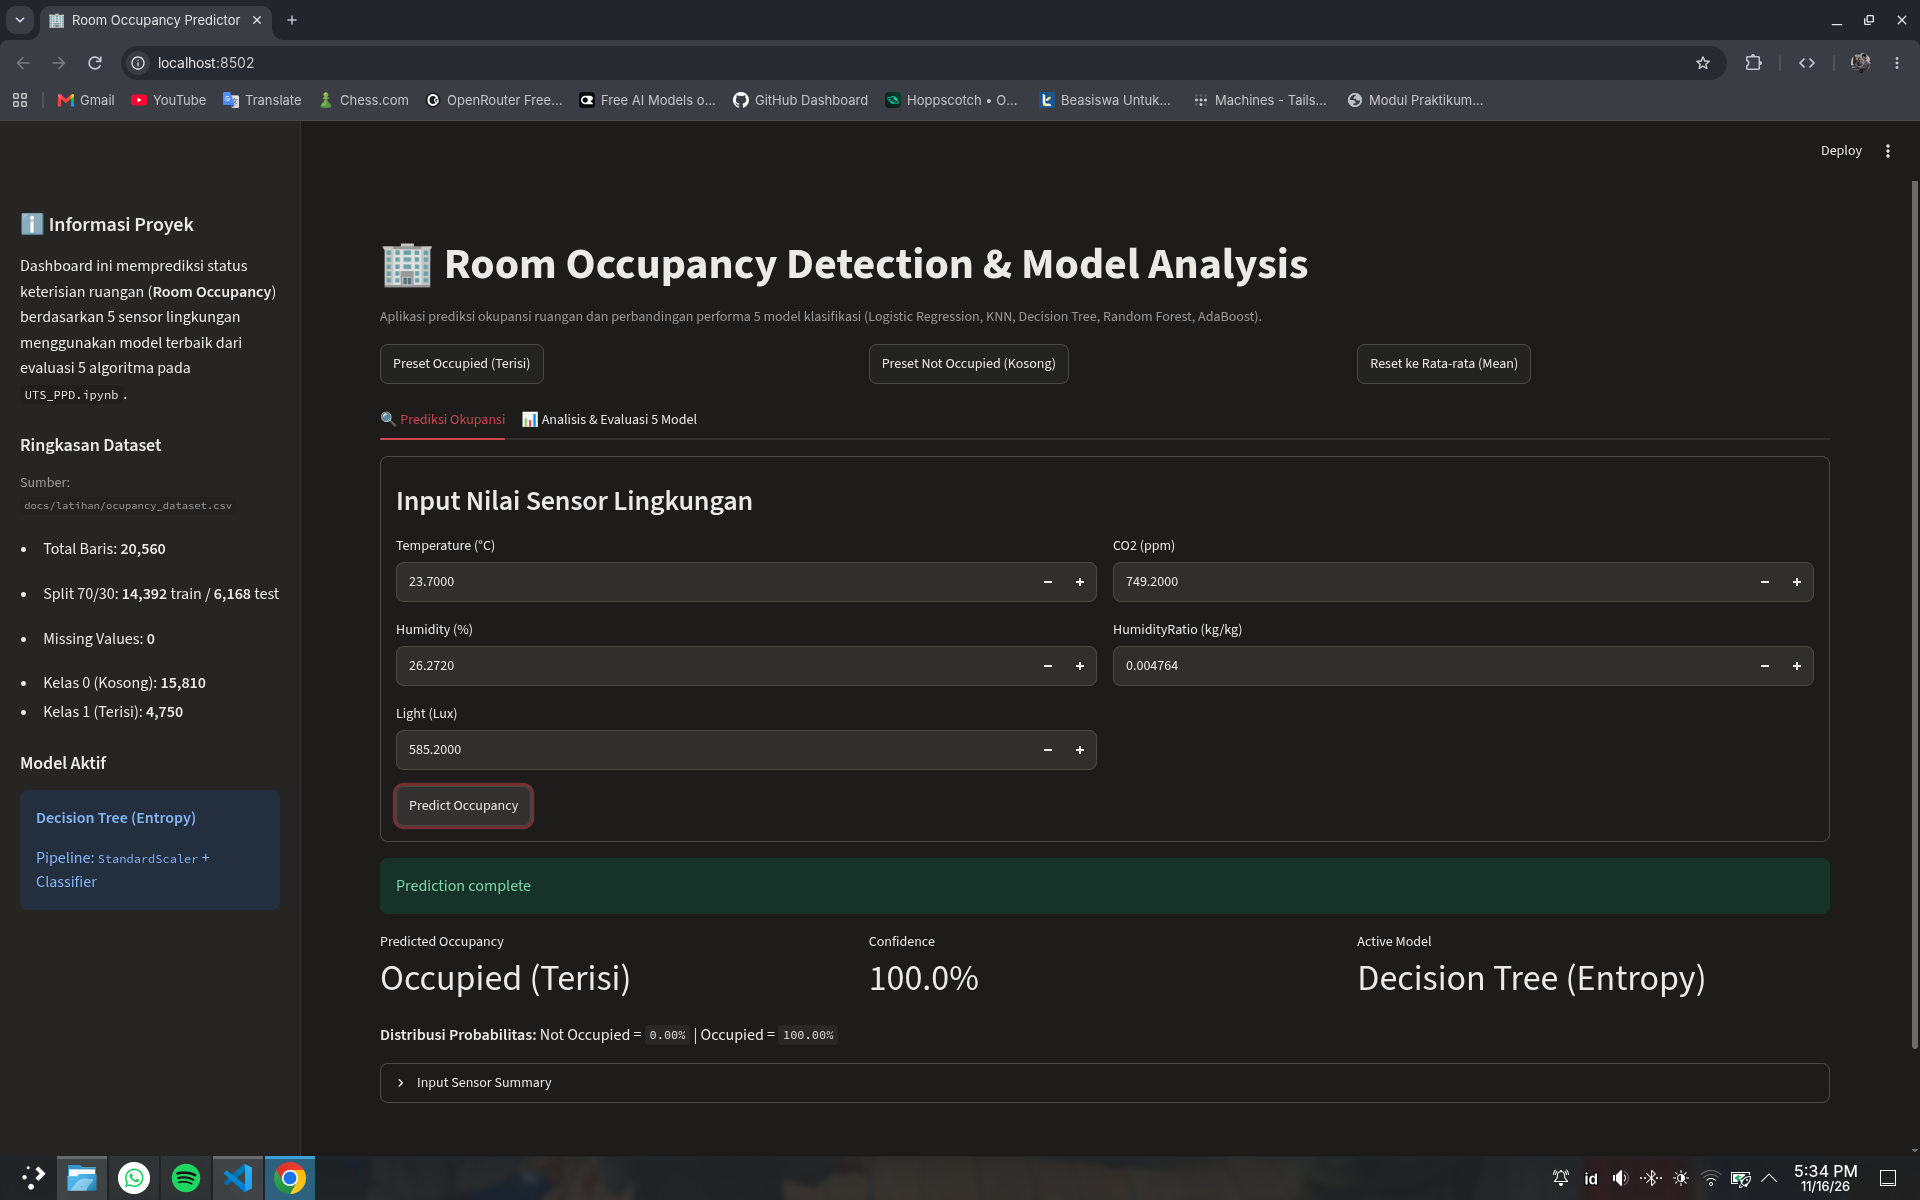
\includegraphics[width=0.8\textwidth]{resource/dokumentasi/tugas-2-hasil-prediksi-occupancy-streamlit.png}
  \caption{Visualisasi Hasil Estimasi Deteksi Keterisian Ruangan dan Pengukur Keyakinan Model}
  \label{fig:tugas-hasil-prediksi-occupancy-streamlit-2}
\end{figure}

\par \textbf{Analisis:} Pada Gambar \ref{fig:tugas-hasil-prediksi-occupancy-streamlit-2}, ketika tombol preset ruangan terisi ditekan (\path{Light = 585.2 Lux}, \path{CO2 = 749.2 ppm}), model \texttt{Decision Tree} langsung menghasilkan inferensi berstatus \textbf{\texttt{RUANGAN TERISI (OCCUPIED)}} dengan tingkat kepastian \textbf{$100{,}0\%$}. Antarmuka Streamlit memvisualisasikan hasil tersebut secara dinamis melalui bilah kemajuan berwarna (\textit{confidence meter} $1{,}0$), kartu metrik probabilitas per kelas, serta tabel komparasi parameter masukan terhadap batas toleransi sensor yang membantu pengguna memvalidasi kewajaran data sensor secara langsung.

\subsection{Analisis Komparatif Paradigma Deployment: Web Service (Flask) vs. Data Application (Streamlit)}

\par Praktikum penambangan data modul ke-10 dan ke-11 memperlihatkan dua paradigma \textit{model deployment} yang memiliki karakteristik, keunggulan, dan skenario pemanfaatan yang sangat berbeda dalam siklus rekayasa perangkat lunak. Flask mewakili paradigma \textit{traditional web micro-framework} berbasis layanan REST/HTTP, sedangkan Streamlit mewakili paradigma \textit{reactive data application framework} berbasis status komponen Python murni. Perbandingan komprehensif kedua teknologi ini dirangkum pada Tabel \ref{tab:komparasi-flask-streamlit}.

\begin{table}[H]
  \centering
  \renewcommand{\arraystretch}{1.25}
  \resizebox{\textwidth}{!}{%
    \begin{tabular}{|l|p{6.5cm}|p{6.5cm}|}
      \hline
      \textbf{Dimensi Perbandingan} & \textbf{Layanan Web Mikro (Flask)} & \textbf{Aplikasi Data Reaktif (Streamlit)} \\ \hline
      Paradigma Eksekusi & \textit{Request--Response Lifecycle} berbasis rute HTTP eksplisit (\texttt{GET}, \texttt{POST}) & \textit{Script Rerun Execution Model} berbasis graf ketergantungan (\textit{Reactive DAG}) \\ \hline
      Arsitektur \& Bahasa & Multibahasa: Python (\textit{backend logic}) + Jinja2 (HTML) + CSS + JavaScript (\textit{client UI}) & Python murni: antarmuka dideklarasikan langsung bersama logika inferensi tanpa menulis HTML/JS \\ \hline
      Manajemen Status (\textit{State}) & \textit{Stateless} secara alami; membutuhkan HTTP \textit{cookies}, sesi server, atau basis data & \textit{Stateful} terkelola melalui memori sesi server (\texttt{st.session\_state}) lintas \textit{rerun} \\ \hline
      Optimasi Memori Artefak & Dimuat ke variabel global modul saat inisialisasi server (\textit{startup}) & Dikelola secara deklaratif menggunakan dekorator \texttt{@st.cache\_resource} dan \texttt{@st.cache\_data} \\ \hline
      Kecepatan Pembuatan Prototipe & Moderat; memerlukan perancangan templat HTML, form handling, dan styling manual & Sangat cepat; widget UI, layout kolom, tabs, dan visualisasi dataframe tersedia bawaan \\ \hline
      Fleksibilitas Desain Antarmuka & Sangat tinggi; pengembang bebas memodifikasi DOM, CSS framework, dan script frontend & Terbatas pada ekosistem komponen dan struktur tata letak bawaan Streamlit \\ \hline
      Kemampuan Integrasi API & Sangat luwes; dapat berfungsi ganda sebagai penyedia RESTful API (JSON) untuk aplikasi mobile/web & Dirancang khusus untuk konsumsi pengguna manusia via peramban; kurang ideal sebagai REST API murni \\ \hline
      Skenario Penggunaan Utama & Layanan mikrosistem produksi, integrasi antarsistem skala besar, sistem dengan kebutuhan kustom UI kompleks & Eksplorasi data interaktif, \textit{internal business dashboard}, demo model machine learning, dan \textit{rapid prototyping} \\ \hline
    \end{tabular}%
  }
  \caption{Perbandingan Paradigma Arsitektur \textit{Model Deployment}: Web Service (Flask) vs. Data Application (Streamlit)}
  \label{tab:komparasi-flask-streamlit}
\end{table}

\par \textbf{Analisis Sintesis Paradigma:} Mengacu pada analisis Tabel \ref{tab:komparasi-flask-streamlit}, pemilihan antara Flask dan Streamlit dalam proyek penambangan data bergantung pada tujuan akhir produk perangkat lunak. Streamlit memberikan efisiensi yang tak tertandingi pada fase eksplorasi, evaluasi stakeholder, dan pembuatan \textit{dashboard} internal berkat kemampuannya memadukan data, model, dan kontrol visual hanya dengan beberapa baris kode Python. Mekanisme \texttt{@st.cache\_resource} dan \texttt{st.session\_state} mengeliminasi kerumitan pengelolaan sesi HTTP dan sinkronisasi berkas templat. Sebaliknya, apabila model ditargetkan menjadi mesin inferensi skala produksi yang melayani ratusan aplikasi klien pihak ketiga (\textit{multi-platform clients}) melalui kontrak data JSON terstandarisasi, Flask menjadi pilihan yang lebih tangguh dan terukur karena memisahkan secara tegas antara lapisan presentasi dan lapisan logika bisnis.

\section{Kesimpulan}

\par Berdasarkan seluruh rangkaian eksperimen, perancangan sistem, dan pengujian implementasi \textit{model deployment} yang telah dilaksanakan pada pertemuan ke-10 (Flask) dan pertemuan ke-11 (Streamlit), dapat dirumuskan beberapa kesimpulan pokok sebagai berikut:
\begin{enumerate}[label=\arabic*.]
  \item \textit{Model deployment} merupakan fase krusial dalam siklus hidup penambangan data (\textit{Machine Learning Lifecycle}) yang menjembatani kesenjangan antara model prediktif statis hasil pelatihan di lingkungan \textit{notebook} dengan pemanfaatan nyata oleh pengguna akhir melalui antarmuka web interaktif dan terstandarisasi.
  \item Pemanfaatan teknik serialisasi Scikit-Learn menggunakan pustaka \texttt{joblib} terbukti sangat efektif untuk mengemas model tunggal maupun rangkaian \texttt{Pipeline} (termasuk tahapan \texttt{StandardScaler}) menjadi artefak biner permanen (\texttt{.model} atau \texttt{.joblib}), sehingga proses \textit{deserialization} saat server dimulai dapat dilakukan secara instan tanpa mengulang komputasi pelatihan.
  \item Implementasi \textit{model deployment} menggunakan \textit{framework} Flask berhasil merealisasikan arsitektur \textit{request-response} berbasis HTTP untuk prediksi penyakit Hepatitis C (\path{hcvdat0.csv}, $12$ fitur klinis) pada port \texttt{5000} dan \textit{dashboard} komparatif \textit{Room Occupancy Detection} (\path{ocupancy_dataset.csv}, $20.560$ data, model terbaik Decision Tree dengan akurasi $99{,}09\%$) pada port \texttt{5001} lengkap dengan validasi kode status \texttt{HTTP 400}.
  \item Implementasi \textit{model deployment} menggunakan \textit{framework} Streamlit menghadirkan arsitektur aplikasi data reaktif (\textit{reactive data application}) berbasis Python murni yang mempercepat perancangan antarmuka visual prediksi Hepatitis C pada port \texttt{8501} serta \textit{dashboard} multi-tab analitik keterisian ruangan pada port \texttt{8502} dengan pemanfaatan optimal \texttt{@st.cache\_resource} untuk efisiensi memori dan \texttt{st.session\_state} untuk fitur \textit{preset} skenario uji.
  \item Sintesis komparatif menunjukkan bahwa Flask unggul dalam hal fleksibilitas arsitektur, kustomisasi antarmuka pengguna berbasis templat web, serta penyediaan antarmuka layanan RESTful skala produksi, sedangkan Streamlit unggul secara signifikan dalam kecepatan \textit{prototyping}, integrasi visualisasi data analitik, dan efisiensi penulisan kode tanpa membutuhkan keahlian terpisah pada teknologi \textit{frontend} (HTML/CSS/JS).
\end{enumerate}

\par Repositori Proyek Praktikum:
\begin{itemize}
  \item Repositori Deployment Flask: \path{deploy-flask/} (Latihan pada \path{deploy-flask/latihan/} dan Tugas pada \path{deploy-flask/tugas/}).
  \item Repositori Deployment Streamlit: \path{deploy-streamlit/} (Latihan pada \path{deploy-streamlit/latihan/} dan Tugas pada \path{deploy-streamlit/tugas/}).
\end{itemize}

\section{Daftar Pustaka}
\printbibliography[heading=none]

\end{document}
